% 第4章重构版：现代网络优化技术
% 使用book-writer v2.0 skill：故事化讲解 + Problem→Insight→Design→Proof→Analysis
% 整合AWS SRD、Google Espresso和行业技术文档

\section{现代网络优化技术}\label{sec:modern-optimization}

\begin{quote}
\textit{"网络设备应该是可编程的，就像计算机一样。"}

——这是P4语言设计者的核心信念，也是本章所有技术故事的共同主线。
\end{quote}

在过去的十年里，数据中心网络经历了一场从"硬件定义"到"软件定义"的深刻变革。这场变革不仅仅是技术层面的升级，更是一场思维方式的革命——我们开始把网络设备视为可编程的计算机，而非固定的功能盒子。

本章将讲述六个相互关联的技术故事：
\begin{itemize}
    \item \textbf{AWS SRD}：为什么TCP不适合云数据中心？
    \item \textbf{Google Espresso}：动态边缘路由的革命
    \item \textbf{P4可编程网络}：从固定功能交换机到"开放厨房"
    \item \textbf{eBPF/Cilium}：内核可编程性的革命
    \item \textbf{DPU/SmartNIC}：数据中心计算的第三支柱
    \item \textbf{CXL内存互联}：打破内存墙的新解法
\end{itemize}

这些技术看似独立，实则共享同一个核心理念：\textbf{可编程性}。它们共同描绘了一幅数据中心网络演进的全景图——从封闭到开放，从通用到专用，从集中到分布。

\begin{researchtree}{现代网络优化技术演进 (2014-)}
\treelevel{传输协议革新}
    \treeitem{AWS SRD (2020)}
    \treeitem{Google Falcon (2023)}
    \treeitem{RDMA/RoCEv2演进}
\treelevel{边缘路由SDN}
    \treeitem{Google Espresso (2017)}
    \treeitem{Facebook Edge Fabric (2017)}
    \treeitem{BGP-EPE标准演进}
\treelevel{可编程数据平面}
    \treeitem{P4语言 (SIGCOMM 2014)}
    \treeitem{Intel Tofino可编程芯片 (2016)}
    \treeitem{INT带内网络遥测}
\treelevel{内核可编程性}
    \treeitem{eBPF扩展 (Linux 3.18+)}
    \treeitem{XDP快速路径 (Linux 4.8+)}
    \treeitem{Cilium容器网络 (2016)}
\treelevel{基础设施处理器}
    \treeitem{AWS Nitro架构 (2017)}
    \treeitem{NVIDIA BlueField DPU (2018)}
    \treeitem{Intel IPU (2020)}
\treelevel{内存互联技术}
    \treeitem{CXL 1.0/1.1 (2019)}
    \treeitem{CXL 2.0 内存池化 (2020)}
    \treeitem{CXL 3.0/3.1 Fabric能力 (2022-2024)}
\end{researchtree}

% ============================================================
\subsection{AWS SRD：为云数据中心重塑传输协议}
% ============================================================

\subsubsection{Problem：TCP在云数据中心的困境}

想象你正在参加一场接力赛跑，规则却很奇怪：每位选手必须等前一棒完全跑完才能起跑。更糟糕的是，如果某一棒不慎摔倒，全队必须等待整整两分钟才能继续。这听起来荒谬，但这正是TCP协议在数据中心中的真实写照。

TCP诞生于1974年，为广域网设计，它有两个核心假设：
\begin{enumerate}
    \item 网络是不可靠的，丢包是常态
    \item 带宽时延积（BDP）较大，需要累积确认
\end{enumerate}

这些假设在互联网环境中完全合理，但在现代云数据中心中却成为性能瓶颈：

\textbf{1. 队头阻塞（Head-of-Line Blocking）}

TCP保证严格的有序交付。当单个数据包丢失时，后续所有已到达的数据包都必须等待重传完成才能交付给应用。在云数据中心微秒级RTT环境下，这种等待代价极其高昂。

\textbf{2. 毫秒级重传超时}

传统TCP的最小重传超时（RTO）为200毫秒（RFC 6298）。但在数据中心内部，RTT通常只有几十微秒。这意味着当丢包发生时，TCP会等待比实际需要长100倍的时间才进行重传。

\textbf{3. ECMP哈希冲突}

现代数据中心使用等价多路径（ECMP）来利用丰富的网络拓扑。TCP使用五元组哈希选择路径，当多个流哈希到同一路径时，会造成热点。TCP被"锁定"在拥塞路径上，无法动态切换。

\textbf{4. 单路径限制}

传统TCP每个连接只能使用单条路径，即使在多路径丰富的数据中心网络中也是如此。这导致网络利用率低下，无法充分利用拓扑冗余。

\textbf{AWS的实际挑战}：

AWS运行着全球最大的云基础设施，支撑着从Web服务到AI训练的各类工作负载。在2020年前后，他们发现了一个严峻问题：

\begin{quote}
\textit{随着HPC和分布式机器学习工作负载的增长，TCP的性能瓶颈日益突出。这些工作负载采用Bulk Synchronous Parallel（BSP）计算模型，整个集群的性能取决于最慢节点的完成时间。}

\textit{TCP的尾延迟问题（tail latency）在这种场景下被放大——只要有一个连接经历丢包，就会拖慢整个同步点。}
\end{quote}

他们意识到：\textbf{在云数据中心环境中，我们需要一种全新的传输协议，从根本上重新思考可靠性与有序性的关系。}

\subsubsection{Insight：可靠但无序的设计哲学}

AWS工程师开始思考一个根本性问题：

\begin{quote}
\textit{严格的有序交付真的是必须的吗？}
\end{quote}

经过深入分析，他们发现：
\begin{itemize}
    \item 在MPI（Message Passing Interface）中，只有使用相同标签的消息才需要有序
    \item 在机器学习参数同步中，不同层之间的参数更新是独立的
    \item 在NVMe-oF存储访问中，不同IO请求天然独立
\end{itemize}

这启发他们思考一种全新的传输范式：
\textbf{Reliable but Out-of-Order}（可靠但无序）

\begin{analogy}{TCP vs SRD的快递比喻}
\textbf{TCP}像是一个要求严格按顺序签收的快递服务。即使你的5个包裹都已到达仓库，如果第3个包裹延误，你也必须先等待它到达，才能领取第4、第5个包裹。

\textbf{SRD}像是智能快递柜系统。每个包裹独立送达，你可以随时领取已到达的包裹，无需等待其他包裹。系统保证每个包裹最终都会到达，但不保证到达顺序。
\end{analogy}

这一设计哲学的核心是\textbf{关注点分离}：
\begin{itemize}
    \item 传输层负责\textbf{可靠性}：确保每个数据包最终到达
    \item 应用层负责\textbf{排序}：根据应用语义决定是否需要排序
\end{itemize}

通过这种分离，SRD实现了：
\begin{enumerate}
    \item 消除队头阻塞：丢包只影响该包所属的消息
    \item 并行传输：多条消息可以同时传输，互不干扰
    \item 灵活重排：应用可以根据需要选择重排策略
\end{enumerate}

\subsubsection{Design：多路径包喷洒与主动拥塞控制}

基于可靠但无序的设计哲学，AWS团队设计了\textbf{SRD}（Scalable Reliable Datagram，可扩展可靠数据报）协议。

\textbf{1. 多路径包喷洒（Multipath Packet Spraying）}

SRD最具创新性的设计是多路径传输。不同于TCP的单路径限制，SRD会：

\begin{itemize}
    \item \textbf{主动喷洒}：将数据包分散到所有可用路径上
    \item \textbf{动态避障}：实时监测各路径拥塞情况，避开拥塞路径
    \item \textbf{快速恢复}：当某路径失效时，立即将流量切换到其他路径
\end{itemize}

\begin{figure}[h]
\centering
\begin{tikzpicture}[
    node distance=0.8cm,
    host/.style={rectangle, draw, fill=blue!20, minimum width=2cm, minimum height=1cm, align=center},
    switch/.style={rectangle, draw, fill=gray!20, minimum width=1.5cm, minimum height=0.8cm, align=center},
    path/.style={->, thick, color=blue!60},
    packet/.style={circle, fill=red!60, minimum size=0.3cm, inner sep=0pt},
    label/.style={font=\small}
]
    % Sender
    \node[host] (sender) {发送端\\SRD};
    
    % Top switches
    \node[switch, right=2cm of sender, yshift=1.5cm] (sw1) {交换机 A};
    \node[switch, right=2cm of sender, yshift=-1.5cm] (sw2) {交换机 B};
    
    % Middle switches
    \node[switch, right=2cm of sw1] (sw3) {交换机 C};
    \node[switch, right=2cm of sw2] (sw4) {交换机 D};
    
    % Receiver
    \node[host, right=2cm of sw3, yshift=-1.5cm] (receiver) {接收端\\SRD};
    
    % Paths - showing multipath spraying
    \draw[path] (sender.east) -- node[above, sloped, font=\scriptsize] {Pkt 1,3} (sw1.west);
    \draw[path] (sender.east) -- node[below, sloped, font=\scriptsize] {Pkt 2,4} (sw2.west);
    
    \draw[path] (sw1.east) -- (sw3.west);
    \draw[path] (sw1.east) -- (sw4.west);
    \draw[path] (sw2.east) -- (sw3.west);
    \draw[path] (sw2.east) -- (sw4.west);
    
    \draw[path] (sw3.east) -- (receiver.west);
    \draw[path] (sw4.east) -- (receiver.west);
    
    % Packets visualization
    \node[packet, right=0.8cm of sender, yshift=0.8cm] (p1) {\tiny1};
    \node[packet, right=1.2cm of sender, yshift=0.5cm] (p3) {\tiny3};
    \node[packet, right=0.8cm of sender, yshift=-0.8cm] (p2) {\tiny2};
    \node[packet, right=1.2cm of sender, yshift=-0.5cm] (p4) {\tiny4};
    
    % Reordering at receiver
    \node[right=0.5cm of receiver, font=\scriptsize, align=left] {无序到达:\\3-1-4-2\\应用层重排};
    
    % Legend
    \node[below=1.5cm of sender, font=\small, align=left] {\textbf{SRD特点:}\\• 单流使用多路径\\• 主动喷洒避免热点\\• 动态避障};
\end{tikzpicture}
\caption{SRD多路径包喷洒示意图}
\label{fig:srd-multipath}
\end{figure}

如图~\ref{fig:srd-multipath}所示，SRD允许单个流的数据包通过多条路径并行传输，即使数据包无序到达，应用层也可以根据需要进行重排。

\textbf{2. 发送端控制ECMP}

传统ECMP由交换机根据流哈希决定路径，这导致：
\begin{itemize}
    \item 流一旦建立就被"锁定"在特定路径
    \item 无法避免哈希冲突导致的热点
    \item 对网络拥塞反应迟钝
\end{itemize}

SRD采用了截然不同的方法——\textbf{发送端控制ECMP}：
\begin{itemize}
    \item SRD在发送端操纵数据包封装（如修改外层UDP端口），影响交换机的哈希计算
    \item 发送端主动选择每条数据包的路径
    \item 可以实时根据拥塞情况调整路径分配
\end{itemize}

\textbf{3. 主动拥塞控制}

传统TCP采用\textbf{反应式}拥塞控制：检测到丢包或ECN标记后才降低发送速率。SRD采用\textbf{主动式}策略：

\begin{itemize}
    \item 持续监测各路径的队列深度和延迟
    \item 仅在预估网络管道有足够容量时才发送数据包
    \item 保持队列最小化，减少排队延迟
\end{itemize}

\textbf{4. Nitro硬件卸载}

SRD被实现在AWS Nitro网络卡中，而非主机软件栈：
\begin{itemize}
    \item 避免操作系统和Hypervisor的性能干扰
    \item 实现亚毫秒级重传（相比TCP的200ms RTO）
    \item 提供确定性的低延迟性能
\end{itemize}

\subsubsection{Proof：HPC与AI训练的性能飞跃}

SRD通过AWS Elastic Fabric Adapter（EFA）向客户暴露接口，支持标准MPI和NCCL。

\begin{table}[h]
\centering
\caption{SRD vs TCP性能对比}
\begin{tabular}{lccc}
\toprule
\textbf{指标} & \textbf{虚拟化+TCP} & \textbf{虚拟化+SRD} & \textbf{改善} \\
\midrule
P99.9延迟 & 数毫秒 & 数十微秒 & 85\%降低 \\
单流带宽 & ~5 Gbps & 25 Gbps & 5倍提升 \\
多路径利用 & 单路径 & 64路径 & 质的飞跃 \\
重传延迟 & 200ms (RTO) & 亚毫秒 & ~100倍提升 \\
拥塞控制 & 反应式 & 主动式 & 延迟降低10倍 \\
CPU开销 & 显著 & <1\% & 硬件卸载 \\
\bottomrule
\end{tabular}
\end{table}

\textbf{实际应用效果}：

\begin{itemize}
    \item \textbf{第二代EFA}在相同P4d硬件上，小型和中型消息性能提升高达50\%，大型消息提升10\%
    \item 128 GPU集群测试中，PyTorch FSDP训练性能提升18\%，Megatron-LM提升8\%
    \item 加速器小型集体操作通信时间改善50\%
    \item EBS io2 Block Express通过SRD实现次毫秒级延迟，PostgreSQL写入延迟降低3.47倍
\end{itemize}

\subsubsection{Analysis：垂直整合的技术价值}

SRD的成功展示了云厂商\textbf{垂直整合}的技术价值：

\begin{itemize}
    \item \textbf{网络拓扑可控}：AWS设计并运营自己的数据中心网络，可以针对其拓扑优化协议
    \item \textbf{硬件协同}：SRD与Nitro卡深度集成，实现OS-bypass
    \item \textbf{端到端优化}：从网卡到交换机到拓扑，全栈可控
\end{itemize}

然而，SRD是AWS专有技术，依赖于Nitro硬件。这引出一个问题：\textbf{在更广阔的互联网边界，如何实现类似的灵活性和可编程性？}

Google Espresso提供了另一个视角。

% ============================================================
\subsection{Google Espresso：动态边缘路由的革命}
% ============================================================

\subsubsection{Problem：静态BGP的局限性}

想象你是一个跨国物流公司的调度主管，你的工作是确保包裹以最快速度送达全球客户。但有一个问题：你只能使用一张十年前绘制的地图，而且不能实时调整路线。即使某条高速公路发生严重拥堵，你也只能按照既定路线发送所有车辆。

这正是传统互联网边缘路由面临的困境。

\textbf{BGP（Border Gateway Protocol）}是互联网的路由协议，自1994年成为标准以来，其核心机制几乎没有变化：
\begin{itemize}
    \item 基于策略和属性的路径选择
    \item 本地视图决策，缺乏全局优化
    \item 收敛时间以分钟计，故障恢复缓慢
    \item 无法感知应用层的服务质量需求
\end{itemize}

在云时代，这些问题变得尤为突出：

\textbf{1. 无法感知应用需求}

传统BGP只基于IP前缀做决策。但不同应用对网络质量的需求截然不同：
\begin{itemize}
    \item 视频流需要高带宽、可容忍一定延迟
    \item 实时游戏需要低延迟、低抖动
    \item 网页浏览对两者都有要求
\end{itemize}

BGP无法区分这些流量类型，也就无法进行针对性优化。

\textbf{2. 本地最优非全局最优}

每个路由器独立做决策，基于本地可见信息选择"最佳"路径。但这种局部最优往往导致全局次优——A路由器选择的路径可能与B路由器选择的路径在网络核心处产生拥塞。

\textbf{3. 故障恢复缓慢}

当链路或路由器故障时，BGP需要传播路由撤销、重新计算最优路径、更新路由表。这个过程可能需要数分钟，对于YouTube、Gmail等服务而言是不可接受的。

\textbf{4. 链路利用率不均}

由于静态路由和ECMP的局限性，某些出口链路可能拥塞，而其他链路却空闲。Google发现，传统BGP只能利用约70\%的实际可用容量。

\begin{quote}
\textit{"那些路由协议的目标只是找到一条从源到目的地的路径，而不是找到最佳路径，也不是动态调整路径。"}

——Google Fellow Amin Vahdat
\end{quote}

他们意识到：\textbf{互联网边缘需要一场软件定义的革命，将全局视角和实时优化引入路由决策。}

\subsubsection{Insight：SDN从内部网络延伸到互联网边界}

2012年，Google展示了B4——业界第一个SDN广域网，连接其全球数据中心。B4的成功证明了SDN在大规模网络中的可行性。

但B4解决的是Google\textbf{内部}网络的流量工程问题。一个更大的挑战摆在面前：\textbf{能否将SDN延伸到互联网边缘，改造与ISP和其他网络对等互联的Peering Fabric？}

这引出了Espresso的核心洞察：

\begin{analogy}{路由控制的演进}
\textbf{传统BGP}像是分散的地方政府，每个路由器自己做决策，没有全局协调。

\textbf{Espresso}像是中央集权的联邦制：全局控制器制定整体战略，本地控制器处理战术执行，路由器（交换机）只负责执行最简单的转发。
\end{analogy}

Espresso的设计原则：
\begin{enumerate}
    \item \textbf{层次化控制平面}：全局控制器（Global Controller）负责跨区域的流量工程，本地控制器（Location Controller）处理PoP内的实时事件
    \item \textbf{Fail-Static}：任何组件故障，系统都能继续以故障前的状态运行
    \item \textbf{软件可编程}：通过软件而非硬件实现路由逻辑，加速创新
\end{enumerate}

\subsubsection{Design：解耦路由器，软件定义Peering}

Espresso的核心创新是\textbf{解耦Peering路由器}：

\begin{figure}[h]
\centering
\begin{tikzpicture}[
    node distance=0.6cm,
    box/.style={rectangle, draw, fill=blue!10, minimum width=3cm, minimum height=0.9cm, align=center},
    sbox/.style={rectangle, draw, fill=green!10, minimum width=2.5cm, minimum height=0.8cm, align=center, font=\small},
    arrow/.style={->, thick},
    label/.style={font=\small\bfseries}
]
    % Global Controller
    \node[box, fill=purple!20] (gc) {全局控制器 (GC)\\全球流量工程};
    
    % Local Controllers
    \node[box, below left=1.2cm and 0.5cm of gc, fill=orange!20] (lc1) {本地控制器 (LC)\\Metro POP 1};
    \node[box, below right=1.2cm and 0.5cm of gc, fill=orange!20] (lc2) {本地控制器 (LC)\\Metro POP 2};
    
    % Host servers
    \node[sbox, below=0.8cm of lc1] (host1) {主机集群\\BGP Speaker};
    \node[sbox, below=0.8cm of lc2] (host2) {主机集群\\BGP Speaker};
    
    % Peering Fabric
    \node[box, below=0.8cm of host1, fill=gray!20] (pf1) {Peering Fabric\\MPLS交换机};
    \node[box, below=0.8cm of host2, fill=gray!20] (pf2) {Peering Fabric\\MPLS交换机};
    
    % Peers
    \node[below=0.5cm of pf1, font=\small] (peer1) {ISP Peers};
    \node[below=0.5cm of pf2, font=\small] (peer2) {ISP Peers};
    
    % Connections
    \draw[arrow] (gc) -- (lc1);
    \draw[arrow] (gc) -- (lc2);
    \draw[arrow, <->] (lc1) -- (host1);
    \draw[arrow, <->] (lc2) -- (host2);
    \draw[arrow, <->] (host1) -- (pf1);
    \draw[arrow, <->] (host2) -- (pf2);
    \draw[arrow] (pf1) -- (peer1);
    \draw[arrow] (pf2) -- (peer2);
    
    % Labels on the side
    \node[right=0.3cm of gc, font=\scriptsize, align=left] {• 应用感知调度\\• 全局优化\\• 跨Metro协调};
    \node[right=0.3cm of lc1, font=\scriptsize, align=left] {• 快速故障恢复\\• BGP会话管理\\• 本地路径计算};
    \node[left=0.3cm of pf1, font=\scriptsize, align=left] {• 简单MPLS转发\\• 无状态交换\\• 解耦控制平面};
\end{tikzpicture}
\caption{Google Espresso架构图}
\label{fig:espresso-arch}
\end{figure}

如图~\ref{fig:espresso-arch}所示，Espresso架构包含以下关键组件：

\textbf{1. 主机上运行BGP（Software BGP）}

传统路由器的BGP功能被转移到标准服务器上运行：
\begin{itemize}
    \item 使用自研\textbf{Raven} BGP协议栈（替代Quagga）
    \item 多核Scale-out架构，支持更多Peer
    \item BGP会话分散到多台服务器，单点故障只影响少量会话
\end{itemize}

\textbf{2. 主机存储完整Internet路由表}

每台主机维护完整的Internet转发表（约190万Prefix）：
\begin{itemize}
    \item IPv4使用Compressed Multibyte Trie算法
    \item IPv6使用Binary Trie
    \item 仅占用1.2GB内存，CPU占用率2-3\%
\end{itemize}

\textbf{3. Peering Fabric简化}

Peering设备从复杂的路由器简化为\textbf{MPLS交换机}：
\begin{itemize}
    \item 只需支持MPLS标签交换
    \item 大Buffer、QoS能力强
    \item 小型FIB表，无需存储完整Internet路由
\end{itemize}

\textbf{4. MPLS-over-GRE隧道}

数据流：
\begin{enumerate}
    \item 主机根据GC计算的FIB，选择最佳出口路由器/端口
    \item 数据包被封装为IP-GRE（目标指向PF）+ MPLS（标识Peering端口）
    \item PF解封装，根据MPLS标签转发到对应Peer
\end{enumerate}

\textbf{5. 层次化控制器}

\begin{itemize}
    \item \textbf{全局控制器（GC）}：
    \begin{itemize}
        \item 收集所有Peering设备的BGP路由
        \item 计算应用感知的FIB
        \item 响应L7 Proxy的实时带宽需求
        \item 全局流量工程优化
    \end{itemize}
    
    \item \textbf{本地控制器（LC）}：
    \begin{itemize}
        \item 快速响应本地网络事件（BGP会话故障、端口故障）
        \item 管理BGP Speaker的生命周期
        \item 维护本地Peering端口状态
    \end{itemize}
\end{itemize}

\textbf{6. 主动探测与动态调度}

Espresso不会被动等待拥塞发生：
\begin{itemize}
    \item 主动将少量流量"喷洒"到所有可用路径
    \item 实时测量各路径性能
    \item 根据应用需求（视频/网页/API调用）动态选择最优路径
\end{itemize}

\subsubsection{Proof：生产环境的性能提升}

Espresso于2017年公布时已运行3年多，服务\textbf{20\%}的Google用户流量。

\begin{table}[h]
\centering
\caption{Espresso实际效果}
\begin{tabular}{lc}
\toprule
\textbf{指标} & \textbf{改善} \\
\midrule
相比传统BGP的传输容量 & +13\% \\
链路利用率 & 显著提高 \\
视频Rebuffer率 & 降低35-170\% \\
用户感知延迟 & 显著降低 \\
故障恢复时间 & 从分钟级降至秒级 \\
新特性上线周期 & 从月缩短至周 \\
\bottomrule
\end{tabular}
\end{table}

\textbf{Google成为业界第一个在WAN网络中完全不使用传统路由器的公司}——全网采用Switch/Server架构。

\subsubsection{Analysis：SDN从内部走向边界}

Espresso证明了SDN不仅适用于数据中心内部，也可以应用于互联网边界：

\begin{itemize}
    \item \textbf{解耦创造价值}：将路由器解耦为软件+交换机，实现更灵活的控制
    \item \textbf{全局优化优于本地优化}：全局视角的流量工程显著提升资源利用率
    \item \textbf{应用感知是未来}：网络应该理解应用需求，而非仅基于IP转发
\end{itemize}

与Facebook Edge Fabric（使用BGP Local Preference）相比，Espresso更彻底地拥抱了SDN理念，虽然开发工作量更大，但实现了真正的应用感知流量工程。

% ============================================================
\subsection{协议对比：TCP vs SRD vs RDMA}
% ============================================================

在了解了SRD和Espresso之后，让我们系统性地比较一下现代数据中心常用的传输协议。

\begin{figure}[h]
\centering
\begin{tikzpicture}[
    node distance=0.5cm,
    protocol/.style={rectangle, draw, fill=blue!10, minimum width=3.5cm, minimum height=1.2cm, align=center},
    feature/.style={rectangle, draw, fill=gray!10, minimum width=2.5cm, minimum height=0.7cm, align=center, font=\small},
    arrow/.style={->, thick}
]
    % Protocols
    \node[protocol, fill=green!20] (tcp) {TCP\\1974};
    \node[protocol, right=0.8cm of tcp, fill=yellow!20] (srd) {SRD\\2020};
    \node[protocol, right=0.8cm of srd, fill=orange!20] (roce) {RoCEv2\\2014};
    \node[protocol, right=0.8cm of roce, fill=purple!20] (ib) {InfiniBand RC\\1999};
    
    % Features comparison
    \node[feature, below=0.5cm of tcp] (tcp1) {可靠有序};
    \node[feature, below=0.2cm of tcp1] (tcp2) {单路径};
    \node[feature, below=0.2cm of tcp2] (tcp3) {软件实现};
    
    \node[feature, below=0.5cm of srd] (srd1) {可靠无序};
    \node[feature, below=0.2cm of srd1] (srd2) {64路径喷洒};
    \node[feature, below=0.2cm of srd2] (srd3) {硬件卸载};
    
    \node[feature, below=0.5cm of roce] (roce1) {可靠有序/无序};
    \node[feature, below=0.2cm of roce1] (roce2) {多路径};
    \node[feature, below=0.2cm of roce2] (roce3) {需要无损以太网};
    
    \node[feature, below=0.5cm of ib] (ib1) {可靠有序连接};
    \node[feature, below=0.2cm of ib1] (ib2) {硬件多路径};
    \node[feature, below=0.2cm of ib2] (ib3) {需要专用HCA};
    
    % Connect
    \draw[arrow] (tcp) -- (tcp1);
    \draw[arrow] (srd) -- (srd1);
    \draw[arrow] (roce) -- (roce1);
    \draw[arrow] (ib) -- (ib1);
\end{tikzpicture}
\caption{传输协议特性对比图}
\label{fig:protocol-compare}
\end{figure}

\begin{table}[h]
\centering
\caption{现代数据中心传输协议全面对比}
\begin{tabular}{p{2.5cm}cccccc}
\toprule
\textbf{特性} & \textbf{TCP} & \textbf{UDP} & \textbf{InfiniBand RC} & \textbf{RoCEv2} & \textbf{SRD} & \textbf{Falcon} \\
\midrule
\textbf{可靠性} & 可靠有序 & 无保证 & 可靠有序 & 依赖网络层 & 可靠无序 & 可靠传输 \\
\textbf{多路径} & 单路径 & 应用决定 & 硬件多路径 & 硬件多路径 & 64路径喷洒 & 硬件多路径 \\
\textbf{延迟} & 数十微秒 & 微秒级 & 微秒级 & 微秒级 & 微秒级 & 微秒级 \\
\textbf{硬件要求} & 无 & 无 & HCA/TCA & 无损以太网 & Nitro卡 & IPU \\
\textbf{部署复杂度} & 低 & 低 & 高 & 中等 & 专有硬件 & 专有硬件 \\
\textbf{适用场景} & 通用Web & 实时游戏 & HPC集群 & AI训练 & 云HPC/ML & Google内部 \\
\bottomrule
\end{tabular}
\end{table}

\subsubsection{场景选择指南}

\textbf{选择TCP当：}
\begin{itemize}
    \item 需要最大兼容性
    \item 广域网传输
    \item 对延迟不敏感的后台任务
\end{itemize}

\textbf{选择SRD当：}
\begin{itemize}
    \item 在AWS上运行HPC或AI训练
    \item 需要超低尾延迟
    \item 使用EFA-enabled实例
\end{itemize}

\textbf{选择RoCEv2当：}
\begin{itemize}
    \item 自建数据中心
    \item 需要RDMA性能但不愿使用InfiniBand
    \item 网络基础设施支持无损以太网（PFC/ECN）
\end{itemize}

\textbf{选择InfiniBand当：}
\begin{itemize}
    \item 顶级超算环境
    \item 极致性能需求
    \item 可以接受专用硬件生态
\end{itemize}

% ============================================================
\subsection{P4可编程网络：从固定菜单到开放厨房}
% ============================================================

\subsubsection{Problem：被困在硬件里的创新}

想象你是一家餐厅的主厨，但你的厨房设备是固定的——烤箱只能设定预设温度，炉灶只有固定火力档位，甚至连刀具都是固定的几种规格。如果你想尝试一种新的烹饪技术，唯一的办法是等待设备厂商推出新型号的厨房设备。

这听起来荒谬，但这正是网络工程师在2010年代面对的现实。

传统网络交换机的数据平面由专用ASIC芯片实现，其功能是\textbf{固定}的。芯片厂商在设计时预定义了支持的协议和处理逻辑：以太网帧如何解析、IP头部如何处理、TCP/UDP如何识别。虽然这些ASIC在特定任务上表现出色，但一旦部署就无法适应新的协议或处理逻辑。

这种僵化性带来的问题在快速变化的数据中心中日益突出：

\begin{itemize}
    \item 当VXLAN、Geneve等新型隧道协议出现时，运营商只能等待下一代芯片支持
    \item 当需要自定义的负载均衡逻辑时，只能依赖CPU进行软件处理，性能大打折扣
    \item 当网络故障需要定位时，传统SNMP、NetFlow提供的聚合统计信息粒度太粗
\end{itemize}

\textbf{软件定义网络（SDN）}部分解决了控制平面的灵活性问题，但数据平面仍然受限于固定功能硬件。OpenFlow协议虽然允许控制器下发流表规则，但支持的匹配字段和动作类型是预先定义的，无法处理更复杂的需求（如深度包检测、自定义协议解析）。

他们意识到：\textbf{如果数据平面可以像软件一样编程，网络创新的速度将从根本上改变。}

\subsubsection{Insight：协议无关的数据平面}

2014年，来自斯坦福大学、英特尔、微软和谷歌的研究人员汇聚在一起，开始思考一个大胆的问题：

\begin{quote}
\textit{我们能否设计一种语言，让网络工程师能够像编写软件一样定义硬件的数据包处理流水线？}
\end{quote}

这个问题背后是一个更深层的洞察：\textbf{协议应该是可定义的，而非硬编码的}。

传统交换机的协议栈是固定的：以太网→VLAN→MPLS→IP→TCP/UDP。但为什么网络设备必须理解这些特定协议？为什么不能让用户定义自己的协议格式？为什么不能在一个交换机上同时支持传统以太网和全新设计的协议？

这启发他们思考一种全新的网络编程范式：
\begin{enumerate}
    \item \textbf{协议无关性}：不预设任何特定网络协议，程序员可以定义任意的包头格式
    \item \textbf{目标无关性}：程序可以在不同硬件上运行——ASIC、FPGA、NPU、甚至软件交换机
    \item \textbf{可重构性}：程序可以在运行时动态加载，无需重启设备
\end{enumerate}

\begin{analogy}{传统交换机 vs P4可编程交换机}
\textbf{传统交换机}就像一台只能播放预置曲目的音乐盒，功能精致但僵化。\\
\textbf{P4可编程交换机}就像一架钢琴，演奏者（网络工程师）可以自由谱写和演奏任何乐曲。
\end{analogy}

\subsubsection{Design：解析-匹配-执行的流水线}

基于这些洞察，研究团队设计出了\textbf{P4}（Programming Protocol-independent Packet Processors）语言。

P4程序定义了三个核心组件，构成了一个完整的数据包处理流水线：

\textbf{1. 解析器（Parser）}

解析器定义了如何从比特流中提取包头字段。它是一个状态机，根据已解析的内容决定下一步解析什么。

\begin{lstlisting}[language=P4, caption=简单的P4解析器示例]
parser Parser(packet_in packet,
              out headers hdr,
              inout metadata meta) {
    state start {
        transition parse_ethernet;
    }
    
    state parse_ethernet {
        packet.extract(hdr.ethernet);
        transition select(hdr.ethernet.etherType) {
            0x0800: parse_ipv4;
            0x86DD: parse_ipv6;
            default: accept;
        }
    }
    
    state parse_ipv4 {
        packet.extract(hdr.ipv4);
        transition accept;
    }
}
\end{lstlisting}

\textbf{2. 控制流水线（Control Pipeline）}

这是P4程序的核心逻辑，由一系列\textbf{匹配-动作表}（Match-Action Tables, MAT）组成。

\begin{figure}[h]
\centering
\begin{tikzpicture}[
    node distance=0.8cm,
    box/.style={rectangle, draw, fill=blue!10, minimum width=2.5cm, minimum height=0.8cm, align=center},
    arrow/.style={->, thick}
]
    % Input
    \node[box, fill=green!20] (parser) {解析器\\Parser};
    
    % Pipeline stages
    \node[box, right=of parser] (mat1) {MAT 1\\L2交换};
    \node[box, right=of mat1] (mat2) {MAT 2\\ACL检查};
    \node[box, right=of mat2] (mat3) {MAT 3\\L3路由};
    \node[box, right=of mat3] (mat4) {MAT 4\\隧道封装};
    
    % Output
    \node[box, right=of mat4, fill=orange!20] (deparser) {逆解析器\\Deparser};
    
    % Arrows
    \draw[arrow] (parser) -- (mat1);
    \draw[arrow] (mat1) -- (mat2);
    \draw[arrow] (mat2) -- (mat3);
    \draw[arrow] (mat3) -- (mat4);
    \draw[arrow] (mat4) -- (deparser);
    
    % Metadata flow
    \node[box, below=0.5cm of mat2, fill=yellow!20, minimum width=8cm] (metadata) {元数据总线：携带包头解析结果和处理状态};
    \draw[arrow, dashed] (metadata) -- (mat1);
    \draw[arrow, dashed] (metadata) -- (mat2);
    \draw[arrow, dashed] (metadata) -- (mat3);
    \draw[arrow, dashed] (metadata) -- (mat4);
\end{tikzpicture}
\caption{P4数据平面流水线架构}
\label{fig:p4-pipeline}
\end{figure}

如图~\ref{fig:p4-pipeline}所示，数据包首先经过解析器提取包头信息，然后通过多级匹配-动作表进行处理，最后由逆解析器重新组装输出。

\textbf{3. 逆解析器（Deparser）}

逆解析器定义输出数据包的重新组装逻辑，包括修改后的包头和原始负载。

\subsubsection{Proof：带内网络遥测的革命}

P4最具创新性的应用之一是\textbf{带内网络遥测}（In-band Network Telemetry, INT）。

\begin{definition}{带内网络遥测（INT）}
让数据包自己携带遥测信息的技术。INT源在数据包中插入遥测指令，沿途网络设备将本地状态信息（时间戳、队列深度、链路利用率等）附加到数据包中，在目的地统一收集分析。
\end{definition}

传统网络监控依赖于SNMP、NetFlow等控制平面机制。这些方法存在局限：
\begin{itemize}
    \item 被动的、聚合的统计信息，难以定位特定流量的具体路径
    \item 采样率限制了精度——高带宽网络中只能采样分析一小部分流量
    \item 控制平面查询本身带来延迟，难以实现实时监控
\end{itemize}

INT采用了一种完全不同的思路：

\begin{enumerate}
    \item \textbf{INT源}（发送端主机或第一跳交换机）在数据包中插入INT首部，包含遥测指令
    \item \textbf{INT传输节点}（中间交换机）根据指令，将本地状态信息添加到数据包中——完全在数据平面完成，无需控制平面介入
    \item \textbf{INT汇聚点}（接收端主机或最后一跳交换机）提取所有遥测数据并上报，原始数据包继续交付
\end{enumerate}

这种设计提供了\textbf{逐包、逐跳、实时}的网络可见性。每一个数据包都携带了它穿越网络时的完整"病历"——经过了哪些节点、在每个节点停留了多久、遇到了多大的队列拥塞。

\begin{table}[h]
\centering
\caption{传统监控 vs INT对比}
\begin{tabular}{lcc}
\toprule
\textbf{特性} & \textbf{传统监控} & \textbf{INT} \\
\midrule
粒度 & 聚合统计 & 逐包追踪 \\
延迟 & 秒级/分钟级 & 纳秒级精度 \\
路径可见性 & 推断 & 精确 \\
开销 & 控制平面查询 & 数据平面内联 \\
定位精度 & 设备级 & 流级 \\
\bottomrule
\end{tabular}
\end{table}

\textbf{Meta的实践}：在FBOSS（Facebook Open Switching System）中，Meta大量使用P4风格的可编程数据平面来实现网络可视化。通过INT技术，运维人员可以精确定位网络拥塞点，追踪特定流量的端到端路径，将故障排查时间从小时级缩短到秒级。

\subsubsection{Analysis：从硬件驱动到软件定义}

P4的出现标志着网络创新范式的根本性转变：

\begin{itemize}
    \item \textbf{快速协议创新}：新协议的部署从"等待硬件升级"变为"加载新程序"，周期从年缩短到天
    \item \textbf{定制化网络功能}：负载均衡、防火墙、DPI等功能可以直接在交换机硬件执行
    \item \textbf{资源优化}：多种网络功能可以在同一硬件上通过软件定义实现，减少设备数量
    \item \textbf{敏捷响应}：网络策略变更从"配置变更+设备重启"简化为"程序热加载"
\end{itemize}

然而，P4也有其局限性。它需要专用的可编程交换芯片（如Intel Tofino），成本高于传统固定功能芯片。此外，P4编程需要专门的技能，学习曲线较陡。

最重要的是，P4解决了\textbf{网络设备}的可编程问题，但数据中心还有另一个庞大的软件栈运行在Linux内核中。如果我们能让内核本身变得可编程呢？

这正是下一个故事的主题。

% ============================================================
\subsection{eBPF/Cilium：内核可编程性的革命}
% ============================================================

\subsubsection{Problem：内核的封闭性困境}

Linux内核是互联网基础设施的基石，但它有一个长期存在的问题：\textbf{封闭性}。

如果你想为内核添加一个新功能——无论是新的网络协议、安全策略还是监控工具——传统上有两条路：
\begin{enumerate}
    \item 向内核社区提交补丁，等待数年可能被合并
    \item 开发内核模块，但一旦出现错误，整个系统可能崩溃
\end{enumerate}

这种困境在云计算时代变得更加尖锐：
\begin{itemize}
    \item 容器密度极高，单节点可能运行数百个Pod
    \item 服务发现变化频繁，iptables规则需要频繁更新
    \item 网络策略越来越复杂，需要L7层感知能力
\end{itemize}

\textbf{iptables的局限性}在这种场景下暴露无遗：

\begin{itemize}
    \item \textbf{线性查找复杂度}：规则是按顺序匹配的链表，Service数量增加时查找时间线性增长
    \item \textbf{规则更新代价}：更新不是原子性的，可能出现短暂服务中断
    \item \textbf{有限的可见性}：难以快速定位网络问题
    \item \textbf{L7能力缺失}：无法基于HTTP路径、gRPC方法进行策略控制
\end{itemize}

他们意识到：\textbf{我们需要一种机制，既能扩展内核功能，又不会影响内核的稳定性和安全性。}

\subsubsection{Insight：安全沙箱与验证器}

1990年代，BSD Unix引入了一个名为BPF（Berkeley Packet Filter）的小工具，用于网络包过滤。它的核心思想很聪明：用户空间程序可以加载一段小型字节码到内核，内核在执行前验证这段代码是安全的（不会无限循环、不会访问非法内存）。

2014年，Linux内核开发者Alexei Starovoitov看到了扩展这个机制的潜力。他意识到：

\begin{quote}
\textit{如果我们将BPF从简单的包过滤扩展为通用的内核虚拟机，会发生什么？}
\end{quote}

这启发他思考\textbf{eBPF}（Extended BPF）的设计：

\begin{enumerate}
    \item \textbf{通用执行环境}：不仅仅是包过滤，可以挂载到内核的任意位置
    \item \textbf{安全验证}：加载前验证程序不会崩溃内核、不会无限循环
    \item \textbf{高效执行}：JIT编译为本地机器码，性能接近原生
    \item \textbf{数据共享}：通过Map机制与用户空间高效交换数据
\end{enumerate}

\begin{analogy}{内核扩展方式的演进}
\textbf{内核模块}像在家里墙上打洞挂画——效果好但风险高，洞打错了可能破坏房屋结构。\\
\textbf{eBPF}像使用无痕挂钩——既能把画挂好，又不会在墙上留下永久痕迹。
\end{analogy}

\subsubsection{Design：Hook点与Map机制}

eBPF的架构围绕两个核心抽象构建：

\textbf{1. Hook点（Hook Points）}

eBPF程序可以挂载到内核的各个关键位置，在特定事件发生时执行：

\begin{figure}[h]
\centering
\begin{tikzpicture}[
    node distance=0.5cm,
    layer/.style={rectangle, draw, fill=blue!10, minimum width=10cm, minimum height=0.8cm, align=center},
    hook/.style={rectangle, draw, fill=red!20, minimum width=2cm, minimum height=0.6cm, align=center, font=\small},
    label/.style={font=\small\bfseries}
]
    % Layers
    \node[layer] (app) {应用程序层};
    \node[layer, below=of app] (socket) {Socket层};
    \node[layer, below=of socket] (tcp) {TCP/UDP层};
    \node[layer, below=of tcp] (ip) {IP层};
    \node[layer, below=of ip] (link) {链路层};
    \node[layer, fill=green!20, below=of link] (nic) {网卡硬件};
    
    % Hook points
    \node[hook, right=0.5cm of app] (kprobe) {kprobe};
    \node[hook, right=0.5cm of socket] (sockops) {sockops};
    \node[hook, right=0.5cm of tcp] (tc) {TC};
    \node[hook, left=0.5cm of ip] (iptables) {iptables};
    \node[hook, right=0.5cm of link] (xdp) {XDP};
    
    % Labels
    \node[label, left=0.2cm of app] (l1) {用户态};
    \node[label, left=0.2cm of socket] (l2) {内核态};
    \node[label, left=0.2cm of nic] (l3) {硬件};
\end{tikzpicture}
\caption{eBPF在内核中的主要Hook点}
\label{fig:ebpf-hooks}
\end{figure}

如图~\ref{fig:ebpf-hooks}所示，eBPF可以在多个层级拦截和处理：

\begin{itemize}
    \item \textbf{XDP}（eXpress Data Path）：网卡驱动层，数据包进入系统的最早点
    \item \textbf{TC}（Traffic Control）：流量控制层，支持入站和出站处理
    \item \textbf{Socket层}：应用程序的Socket接口处
    \item \textbf{kprobe/tracepoint}：内核函数的入口和出口
\end{itemize}

\textbf{2. Map机制}

eBPF Map是内核中的键值存储，用于：
\begin{itemize}
    \item eBPF程序之间共享数据
    \item eBPF程序与用户空间应用通信
    \item 维护跨数据包的状态（如连接跟踪表）
\end{itemize}

Map支持O(1)复杂度的查找，无论数据量多大，查找时间保持恒定。

\subsubsection{Proof：Cilium的云原生网络}

Cilium项目展示了eBPF在云原生网络中的强大能力。

\begin{definition}{Cilium}
基于eBPF的开源容器网络接口（CNI）插件，为Kubernetes提供高性能的网络连接、负载均衡、网络安全和可观测性能力。
\end{definition}

Cilium的核心创新在于使用eBPF替代iptables：

\textbf{1. O(1)复杂度查找}

Cilium将Service IP到后端Pod IP的映射存储在eBPF Map中。当数据包到达时，eBPF程序直接通过哈希查找定位目标，无论集群规模多大，查找时间都保持恒定。相比之下，iptables需要线性遍历规则链。

\textbf{2. 原子性更新}

eBPF Map的更新是原子性的——可以在不影响现有流量的情况下添加或删除条目。Pod扩缩容不会导致服务中断，策略更新可以即时生效。

\textbf{3. Socket层负载均衡}

Cilium的一个独特优化是在Socket层实现负载均衡。当应用程序发起连接时，eBPF程序直接在Socket层面将目标IP替换为后端Pod IP，避免了后续的NAT处理。

\begin{table}[h]
\centering
\caption{iptables vs Cilium/eBPF性能对比}
\begin{tabular}{lcc}
\toprule
\textbf{场景} & \textbf{iptables} & \textbf{Cilium/eBPF} \\
\midrule
Service查找复杂度 & O(n) & O(1) \\
规则更新原子性 & 否 & 是 \\
L7策略支持 & 需Sidecar & 内核直接处理 \\
连接跟踪开销 & 高 & 低 \\
大规模集群延迟 & 显著增加 & 保持低延迟 \\
\bottomrule
\end{tabular}
\end{table}

\textbf{4. Service Mesh演进}

传统Service Mesh使用Sidecar模式——每个Pod中注入一个Envoy代理。这带来显著的资源和延迟开销。Cilium Service Mesh利用eBPF在内核中实现核心功能：
\begin{itemize}
    \item mTLS通过内核中的WireGuard实现
    \item L7流量管理通过节点共享的Envoy代理实现
    \item 可观测性通过Hubble实现，无需额外的代理插桩
\end{itemize}

\subsubsection{Analysis：重新定义内核边界}

eBPF的出现重新定义了内核与用户空间的边界：

\begin{itemize}
    \item \textbf{内核可扩展性}：无需重新编译内核即可添加功能
    \item \textbf{安全保证}：验证器确保程序不会危害系统稳定性
    \item \textbf{高性能}：JIT编译使eBPF程序性能接近原生代码
    \item \textbf{生态繁荣}：bcc、bpftrace等工具极大降低了使用门槛
\end{itemize}

然而，eBPF仍然运行在通用CPU上。当网络流量达到100Gbps甚至400Gbps时，即使是高度优化的eBPF程序也会消耗大量CPU资源。

如果我们能把基础设施任务完全从主机CPU卸载到专用硬件呢？

这就是DPU的故事。

% ============================================================
\subsection{DPU/SmartNIC：数据中心计算的第三支柱}
% ============================================================

\subsubsection{Problem：CPU的"元工作"负担}

想象一家高档餐厅的主厨，他每天的工作时间中有30\%不是在烹饪，而是在处理食材采购单、清洁厨房设备、协调服务员接单——这些都是必要的工作，但它们分散了主厨对核心任务的专注。

这正是现代数据中心中CPU面临的困境。

随着虚拟化、容器化、软件定义网络和安全需求的激增，CPU越来越忙于处理"元工作"（Meta-work）：
\begin{itemize}
    \item 网络协议处理（封装/解封装、校验和计算）
    \item 安全加密/解密（TLS、IPsec）
    \item 存储虚拟化（NVMe-oF、数据压缩）
    \item 虚拟化管理（vSwitch、I/O虚拟化）
\end{itemize}

据统计，在某些云环境中，CPU可能花费30\%甚至更多的周期处理这些基础设施任务。这意味着企业购买的高价CPU，有相当一部分并未用于运行业务应用。

他们意识到：\textbf{基础设施任务应该专用化卸载，让CPU专注于业务逻辑计算。}

\subsubsection{Insight：计算的"三支柱"模型}

回顾计算机体系结构的演进，我们可以看到一个清晰的发展脉络：

\begin{enumerate}
    \item \textbf{CPU时代}：单一处理器处理所有任务
    \item \textbf{CPU+GPU时代}：GPU承担并行计算任务，CPU负责通用计算
    \item \textbf{CPU+GPU+DPU时代}：DPU承担基础设施任务，三种处理器各专其职
\end{enumerate}

这启发架构师们思考一个新的计算模型：

\begin{analogy}{数据中心的"厨房分工"}
\begin{itemize}
    \item \textbf{CPU是主厨}：专注于烹饪（业务逻辑计算）
    \item \textbf{GPU是面点师}：专注于需要大量重复操作的烘焙（并行计算）
    \item \textbf{DPU是后厨主管}：处理食材准备、订单管理、库存监控（基础设施任务）
\end{itemize}
\end{analogy}

\subsubsection{Design：从SmartNIC到DPU的演进}

理解DPU需要厘清它与SmartNIC的关系：

\begin{figure}[h]
\centering
\begin{tikzpicture}[
    node distance=0.3cm,
    stage/.style={rectangle, draw, fill=blue!10, minimum width=3cm, minimum height=1.2cm, align=center},
    arrow/.style={->, thick}
]
    % Stages
    \node[stage, fill=gray!20] (nic) {传统NIC\\基础网络功能};
    \node[stage, right=1.5cm of nic, fill=yellow!20] (smartnic) {SmartNIC\\硬件加速\\可编程流水线};
    \node[stage, right=1.5cm of smartnic, fill=green!20] (dpu) {DPU\\完整基础设施计算机\\独立OS运行};
    
    % Arrows
    \draw[arrow] (nic) -- (smartnic) node[midway, above, font=\small] {功能增强};
    \draw[arrow] (smartnic) -- (dpu) node[midway, above, font=\small] {架构解耦};
    
    % Features
    \node[below=0.3cm of nic, font=\scriptsize, align=center] {ASIC固定功能\\仅数据链路层};
    \node[below=0.3cm of smartnic, font=\scriptsize, align=center] {P4可编程\\RDMA/NVMe-oF卸载};
    \node[below=0.3cm of dpu, font=\scriptsize, align=center] {ARM核心\\完整Linux系统\\安全信任根};
\end{tikzpicture}
\caption{DPU架构演进：从传统NIC到SmartNIC再到DPU}
\label{fig:dpu-evolution}
\end{figure}

如图~\ref{fig:dpu-evolution}所示，DPU的演进经历了三个阶段：

\textbf{1. 传统NIC}
仅负责数据链路层的基本功能，所有高级处理都依赖主机CPU。

\textbf{2. SmartNIC}
增加了可编程流水线和硬件加速引擎，可以卸载部分网络处理任务。但仍依赖主机CPU进行复杂决策。

\textbf{3. DPU}
成为独立的"计算机中的计算机"：
\begin{itemize}
    \item 集成多核ARM处理器，运行完整的操作系统
    \item 独立的控制平面，无需主机参与
    \item 硬件信任根，实现安全隔离
    \item 可以管理虚拟机的网络、存储和安全
\end{itemize}

\textbf{设计权衡：ASIC vs FPGA vs CPU}

不同厂商在DPU设计上做出了不同的技术选择：

\begin{table}[h]
\centering
\caption{DPU实现方案对比}
\begin{tabular}{lccc}
\toprule
\textbf{特性} & \textbf{ASIC} & \textbf{FPGA} & \textbf{通用CPU} \\
\midrule
性能 & 最高 & 高 & 中等 \\
功耗 & 最低 & 中等 & 较高 \\
灵活性 & 低 & 最高 & 高 \\
开发周期 & 长 & 中等 & 短 \\
成本（大规模） & 最低 & 高 & 中等 \\
代表产品 & NVIDIA BlueField & Intel IPU (FPGA) & AMD Pensando \\
\bottomrule
\end{tabular}
\end{table}

\subsubsection{Proof：行业实践与产品路线}

\textbf{NVIDIA BlueField系列}：
\begin{itemize}
    \item BlueField-3集成16个ARM核心、220亿晶体管、16GB DDR5
    \item 支持400Gb/s网络吞吐能力
    \item 与GPU生态紧密集成，支持GPUDirect RDMA
\end{itemize}

\textbf{Intel IPU}：
\begin{itemize}
    \item 采用ASIC+FPGA混合策略
    \item Mount Evans：与Google Cloud合作开发的ASIC IPU
    \item Oak Springs Canyon：基于FPGA的灵活方案
\end{itemize}

\textbf{AWS Nitro架构}：
\begin{itemize}
    \item DPU（Nitro卡）接管主机的所有基础设施功能
    \item 主机CPU可以100\%专注于客户工作负载
    \item 这是DPU理念最早的大规模生产实践
\end{itemize}

\subsubsection{Analysis：数据中心架构的范式转变}

DPU的普及正在从根本上改变数据中心的体系结构：

\begin{enumerate}
    \item \textbf{计算的"三支柱"模型}形成：CPU负责通用计算，GPU负责并行计算，DPU负责基础设施任务
    \item \textbf{算存分离架构}成为主流：计算与存储资源可以物理分离，通过网络高速互联
    \item \textbf{网络成为一等公民}：网络设备从单纯的"转发器"进化为"智能端点"
    \item \textbf{软件定义一切}：数据中心基础设施可以通过软件灵活配置
\end{enumerate}

然而，DPU主要解决的是计算和网络的解耦。数据中心的另一个关键资源——内存——仍然紧密绑定在CPU周围。

如果我们能像扩展存储一样灵活地扩展内存呢？

这就是CXL要解决的问题。

% ============================================================
\subsection{CXL内存互联：打破内存墙}
% ============================================================

\subsubsection{Problem：内存墙与容量瓶颈}

训练一个千亿参数的大语言模型，可能需要TB级别的内存——远超单台服务器所能提供的容量。

传统的解决方案面临诸多限制：
\begin{itemize}
    \item 通过网络组合多台服务器的内存会引入显著的延迟和带宽损失
    \item 一个CPU通常只有4-8个内存通道，每个通道支持有限的DIMM插槽
    \item GPU配备的高带宽HBM内存无法直接共享给CPU使用
\end{itemize}

业界将这一挑战称为"\textbf{内存墙}"（Memory Wall）——计算速度受限于CPU从内存获取数据的速度。

他们意识到：\textbf{内存不应该被物理绑定在CPU周围，而应该是可扩展、可共享的资源池。}

\subsubsection{Insight：缓存一致性互联}

2019年，Intel牵头成立了CXL（Compute Express Link）联盟，提出了一个大胆的想法：

\begin{quote}
\textit{我们能否在保持缓存一致性的前提下，让CPU像访问本地内存一样访问远程内存？}
\end{quote}

这背后的关键洞察是：\textbf{缓存一致性协议可以在多设备间共享}。

传统上，缓存一致性只在CPU内部维护。CXL将其扩展到外部设备：当多个处理器（CPU、GPU、FPGA等）访问同一块内存时，硬件自动维护缓存一致性，无需复杂的软件同步。

\begin{analogy}{内存访问的演进}
\textbf{传统架构}像每个人都只能从自己家的冰箱取食物——方便但容量有限。\\
\textbf{CXL架构}像一个大型的共享厨房——任何人都可以取用自己需要的食物，系统自动保证不会有人拿到变质的食物（缓存一致性）。
\end{analogy}

\subsubsection{Design：三协议栈与设备类型}

CXL协议栈由三个子协议组成：

\begin{figure}[h]
\centering
\begin{tikzpicture}[
    node distance=0.3cm,
    protocol/.style={rectangle, draw, fill=blue!10, minimum width=4cm, minimum height=0.8cm, align=center},
    device/.style={rectangle, draw, fill=green!10, minimum width=3cm, minimum height=0.8cm, align=center},
]
    % Protocols
    \node[protocol] (io) {CXL.io\\传统I/O与配置（PCIe兼容）};
    \node[protocol, below=of io] (cache) {CXL.cache\\设备缓存主机内存的一致性};
    \node[protocol, below=of cache] (mem) {CXL.mem\\主机直接访问设备内存};
    
    % Devices
    \node[device, right=2cm of io] (type1) {Type 1\\网卡等缓存一致性设备};
    \node[device, right=2cm of cache] (type2) {Type 2\\带内存的加速器（GPU）};
    \node[device, right=2cm of mem] (type3) {Type 3\\内存扩展设备};
    
    % Connections
    \draw[->] (io) -- (type1);
    \draw[->] (cache) -- (type2);
    \draw[->] (mem) -- (type3);
\end{tikzpicture}
\caption{CXL协议栈与设备类型}
\label{fig:cxl-protocols}
\end{figure}

如图~\ref{fig:cxl-protocols}所示，三种设备类型分别对应不同的应用场景：

\textbf{Type 1}：网卡等需要缓存一致性但不需要大内存的设备

\textbf{Type 2}：GPU、AI加速器等带大容量内存的加速器，允许CPU直接访问其HBM

\textbf{Type 3}：专用的内存扩展设备，通过CXL.mem扩展系统总内存容量

\textbf{代际演进}：

\begin{table}[h]
\centering
\caption{CXL代际演进}
\begin{tabular}{cll}
\toprule
\textbf{版本} & \textbf{年份} & \textbf{关键特性} \\
\midrule
CXL 1.0/1.1 & 2019 & 基础协议，单节点内互联 \\
CXL 2.0 & 2020 & 引入交换机，支持内存池化 \\
CXL 3.0 & 2022 & Fabric能力，支持4096节点 \\
CXL 3.1 & 2024 & 增强一致性，点对点通信 \\
\bottomrule
\end{tabular}
\end{table}

\subsubsection{Proof：内存池化与AI训练}

\textbf{内存池化场景}：

传统数据中心中，每台服务器配置固定容量的内存，实际利用率往往只有30-40\%。通过CXL内存池化，多台服务器可以共享一个大容量内存池，根据实际需求动态分配内存。

当某个应用需要更多内存时，可以从池中动态获取，而无需物理升级服务器。

\textbf{AI训练场景}：

大模型训练需要TB级内存，而单GPU的HBM容量有限（通常80-96GB）。通过CXL：
\begin{itemize}
    \item GPU可以直接访问通过CXL.mem扩展的大容量内存
    \item CPU和GPU可以共享同一个内存空间，消除不必要的数据拷贝
    \item 支持更大的模型或更大的批次处理，提高吞吐量
\end{itemize}

\textbf{Meta的实践}：

在10X Backbone和AI集群建设中，Meta积极探索CXL技术的应用。通过CXL内存扩展，可以构建更大规模的AI训练集群，支持万亿参数级别的模型训练。

\subsubsection{Analysis：从服务器为中心到资源池为中心}

CXL与DPU的结合，共同推动数据中心架构向"硬件解耦"方向演进：

\begin{itemize}
    \item \textbf{内存与计算的解耦}：内存不再绑定于特定的CPU或服务器
    \item \textbf{异构计算的统一内存空间}：开发者可以使用统一的虚拟地址空间
    \item \textbf{新型内存层级}：热数据驻留本地DDR，温数据存放在CXL扩展内存
    \item \textbf{数据中心即计算机}：整个数据中心的资源可以被视为统一的资源池
\end{itemize}

\begin{table}[h]
\centering
\caption{传统架构 vs 解耦架构对比}
\begin{tabular}{lcc}
\toprule
\textbf{特性} & \textbf{传统架构} & \textbf{解耦架构} \\
\midrule
资源绑定 & 计算+内存紧耦合 & 资源独立扩展 \\
利用率 & 平均30-40\% & 可达70-80\% \\
故障域 & 整机替换 & 组件级替换 \\
扩展性 & 垂直扩展为主 & 水平弹性扩展 \\
成本效率 & 资源碎片化 & 按需分配 \\
\bottomrule
\end{tabular}
\end{table}

% ============================================================
\subsection{总结：可编程性时代的基础设施}
% ============================================================

本章讲述的六个技术故事——SRD、Espresso、P4、eBPF、DPU、CXL——看似独立，实则共享同一个核心理念：\textbf{可编程性}。

\begin{table}[h]
\centering
\caption{现代网络优化技术对比总结}
\begin{tabular}{p{2.5cm}p{2cm}p{2cm}p{2cm}p{1.8cm}p{1.8cm}}
\toprule
\textbf{维度} & \textbf{SRD} & \textbf{Espresso} & \textbf{P4} & \textbf{eBPF} & \textbf{DPU} & \textbf{CXL} \\
\midrule
解决的核心问题 & 云数据中心传输效率 & 互联网边缘路由优化 & 数据平面僵化 & 内核封闭性 & CPU基础设施负担 & 内存墙 \\
核心洞察 & 可靠性与有序性分离 & SDN从内部延伸到边界 & 协议应可定义 & 安全沙箱扩展 & 任务专用化 & 缓存一致性互联 \\
关键技术 & 多路径包喷洒 & 层次化SDN控制 & 匹配动作表 & Hook点+验证器 & ASIC/FPGA加速 & CXL.cache/mem \\
主要受益方 & 云HPC/ML & 云出口流量优化 & 网络工程师 & 系统工程师 & 云服务商 & AI/大数据 \\
\bottomrule
\end{tabular}
\end{table}

它们共同描绘了一幅数据中心网络演进的全景图：

\begin{itemize}
    \item \textbf{性能维度}：网络延迟从毫秒级降至微秒甚至亚微秒级，吞吐量从Gbps提升到Tbps级
    \item \textbf{灵活性维度}：网络创新周期从年缩短到天
    \item \textbf{资源效率维度}：计算、内存、网络资源可以精细匹配工作负载需求
\end{itemize}

\textbf{两大关键趋势}：

\textbf{1. 垂直整合 vs 开源标准化}

SRD展示了云厂商垂直整合的技术价值——从网卡到交换机到拓扑的全栈可控。但这也意味着技术锁定。开源社区正在推动类似能力（如Linux的多路径TCP、DPDK的类似优化），虽然性能可能稍逊，但提供了更好的可移植性。

\textbf{2. 软件定义从内部走向边界}

从B4到Espresso，Google证明了SDN不仅适用于"内部花园"，也可以应用于开放的互联网边界。这开启了一个新的可能性：未来互联网是否可能更加智能、更加应用感知？

\textbf{对未来的启示}：

\begin{enumerate}
    \item \textbf{传输协议创新持续活跃}：SRD、Falcon等专有协议的出现表明，TCP/UDP在特定场景下仍有优化空间
    \item \textbf{软硬协同是必然趋势}：纯软件优化遇到瓶颈，硬件卸载成为标准做法
    \item \textbf{网络可观测性日益重要}：INT、带内遥测等技术让网络黑盒逐渐透明
    \item \textbf{边界正在模糊}：网络、存储、计算的界限日益模糊，统一的可编程基础设施成为目标
\end{enumerate}

展望未来，随着AI模型的持续扩大和实时应用的兴起，数据中心网络将继续向更强的可编程性、更深的软硬件协同、更智能的流量管理方向演进。理解这些技术的工作原理和设计思想，对于设计下一代网络系统具有重要的现实意义。
% Google Cloud WAN与SDN技术补充
% 第4章: 现代优化技术
\subsection{Google Cloud WAN：企业级全球私有网络}

2025年4月，Google宣布将其运营二十余年的全球私有网络向企业开放，推出Cloud WAN服务。这是Google首次将其支撑Search、Gmail、YouTube等核心服务的内部网络基础设施作为独立产品向外部客户提供。

\subsubsection{Cloud WAN的网络基础设施}

\textbf{全球规模数据：}
\begin{itemize}
    \item \textbf{地理覆盖}：200+个国家/地区
    \item \textbf{光纤里程}：200万+英里（含陆地和海底）
    \item \textbf{PoP数量}：202个网络边缘位置
    \item \textbf{海底电缆}：33条私有或共享海底电缆
    \item \textbf{云区域}：42个云区域，127个可用区
    \item \textbf{可靠性SLA}：99.99\%
\end{itemize}

\textbf{关键性能指标：}
\begin{itemize}
    \item 比公共互联网快40\%
    \item 总拥有成本(TCO)降低40\%
    \item 2020-2025年间WAN带宽增长7倍
\end{itemize}

\subsubsection{多分片水平网络架构}

为应对AI时代爆发式增长的流量需求，Google引入了创新的多分片水平网络架构(Multi-shard Horizontal Network Architecture)：

\begin{figure}[htbp]
\centering
\begin{tikzpicture}[scale=0.8, transform shape,
    shard/.style={rectangle, draw, fill=blue!15, minimum width=3cm, minimum height=2cm, align=center},
    control/.style={rectangle, draw, fill=green!15, minimum width=10cm, minimum height=1cm, align=center}
]
% Shards
\node[shard] (s1) at (0,0) {Shard 1\\独立网络实例};
\node[shard] (s2) at (4,0) {Shard 2\\独立网络实例};
\node[shard] (s3) at (8,0) {Shard 3\\独立网络实例};
\node at (12,0) {...};

% Central Control
\node[control] (ctrl) at (6,3) {集中式SDN控制器\\全局拓扑视图 + 流量工程};

% Connections
\draw[->, thick] (ctrl) -- (s1);
\draw[->, thick] (ctrl) -- (s2);
\draw[->, thick] (ctrl) -- (s3);

% Labels
\node at (6,-1.5) {每个分片可独立扩展，类似多ISP冗余};
\end{tikzpicture}
\caption{Google多分片水平网络架构示意图}
\end{figure}

\textbf{架构特点：}
\begin{enumerate}
    \item \textbf{分片独立性}：每个分片是独立的网络实例，可独立运行和维护
    \item \textbf{弹性扩展}：可在分片内部扩展容量，也可增加分片数量
    \item \textbf{冗余设计}：多ISP级别的冗余能力，单分片故障不影响整体服务
    \item \textbf{集中控制}：通过SDN控制器实现全局流量调度和优化
\end{enumerate}

\subsubsection{Cloud WAN核心功能}

\textbf{1. Premium Tier网络}

Premium Tier是Google网络的最高服务级别，确保流量通过地理上最近的网络边缘位置接入：
\begin{itemize}
    \item 流量从源到目的全程在Google私有网络上传输
    \item 通过最近的PoP进入Google网络，减少首跳延迟
    \item 广泛的peering连接，确保最优路径选择
\end{itemize}

\textbf{2. Cross-Cloud Interconnect (CCI)}

Google Cross-Cloud Interconnect为企业多云部署提供专用连接：
\begin{itemize}
    \item 支持10 Gbps和100 Gbps带宽选项
    \item 与AWS、Azure、Oracle等主流云提供商互联
    \item 私有连接，不经过公共互联网
    \item 无跨云数据传输费用（特定合作伙伴）
\end{itemize}

\textbf{3. Cross-Site Interconnect}

2025年新增的Cross-Site Interconnect功能（预览版）提供：
\begin{itemize}
    \item 数据中心之间的Layer 2私有连接
    \item 支持企业构建自己的全球私有网络骨干
    \item 与Google Cloud VPC无缝集成
\end{itemize}

\subsubsection{Cloud WAN与SD-WAN/MPLS对比}

\begin{table}[htbp]
\centering
\caption{企业WAN解决方案对比}
\begin{tabular}{|l|c|c|c|}
\hline
\textbf{特性} & \textbf{传统MPLS} & \textbf{SD-WAN} & \textbf{Cloud WAN} \\
\hline
部署复杂度 & 高（专用线路） & 中（混合模式） & 低（云服务） \\
成本 & 高 & 中 & 低（节省40\%） \\
性能 & 稳定 & 依赖互联网 & 比互联网快40\% \\
全球覆盖 & 有限 & 依赖本地ISP & 200+国家 \\
AI优化 & 无 & 有限 & 原生支持 \\
多云连接 & 复杂 & 中等 & 原生Cross-Cloud \\
\hline
\end{tabular}
\end{table}

\subsection{Google SDN技术演进}

Google是软件定义网络(SDN)技术的先行者和最大规模实践者。从B4 WAN网络到Andromeda虚拟化平台，Google构建了一套完整的SDN技术体系。

\subsubsection{B4：全球SDN WAN网络}

B4是Google连接全球数据中心的私有WAN网络，是SDN技术最成功的商业部署案例之一。

\textbf{B4架构（三层模型）：}

\begin{enumerate}
    \item \textbf{交换机硬件层}：基于商用交换芯片的白盒交换机，专注于高速转发
    \item \textbf{站点控制器层}：运行OpenFlow控制器(OFC)和网络控制应用(NCA)
    \item \textbf{全局控制层}：SDN网关和集中式TE服务器，实现全网流量工程
\end{enumerate}

\textbf{技术创新：}
\begin{itemize}
    \item \textbf{层次化带宽管理(BwE)}：从主机到全局的多级流量控制
    \item \textbf{链路利用率}：通过集中式TE实现98\%+的跨洋光缆利用率
    \item \textbf{故障恢复}：提供"大红色按钮"机制，TE故障时可回退到最短路径
\end{itemize}

\subsubsection{Andromeda：网络虚拟化平台}

Andromeda是Google Cloud的网络虚拟化栈，为GCP提供高性能、隔离和敏捷的网络服务。

\textbf{架构特点：}
\begin{itemize}
    \item \textbf{控制平面}：全局层次结构，维护所有VM和网络状态
    \item \textbf{数据平面}：分布式实现，部分在主机，部分硬件卸载
    \item \textbf{Fast Path}：每包300ns预算的高性能路径
    \item \textbf{Hoverboards}：专用网关处理长尾流量
\end{itemize}

\textbf{性能优化：}
\begin{itemize}
    \item 预留一个物理CPU核心给Andromeda数据平面
    \item 新主机配置预留两个核心以支持更快NIC
    \item 避免在每个主机上安装完整转发表，提升可扩展性
\end{itemize}

\subsubsection{AWS-Google Cloud网络合作 (2025年)}

% AWS网络技术详解
% AWS Nitro System与SRD协议技术详解
% 用于Chapter 3: 交换机设计 和 Chapter 4: 现代优化技术

\section{AWS Nitro系统：硬件卸载的虚拟化架构}

\subsection{Nitro架构演进}

AWS Nitro系统代表了云计算虚拟化架构的根本性重构。传统虚拟化架构中，Hypervisor需要消耗高达25\%的主机计算资源来处理网络、存储和安全任务。Nitro系统通过专用硬件卸载这些功能，将虚拟化开销降至接近零。

\begin{table}[htbp]
\centering
\caption{AWS Nitro系统演进历程}
\begin{tabular}{@{}llll@{}}
\toprule
\textbf{年份} & \textbf{实例} & \textbf{里程碑} & \textbf{性能} \\
\midrule
2013 & C3 & Nitro起步，网络卸载 & 10 Gbps \\
2014 & C4 & 存储卸载(EBS) & - \\
2015 & - & 收购Annapurna Labs & - \\
2017 & C5 & 完整Nitro系统 & 25 Gbps \\
2018 & - & EFA v1发布 & 100 Gbps \\
2020 & - & SRD协议引入 & 微秒级延迟 \\
2022 & - & EFA v2 + ENA Express & 200 Gbps \\
2024 & P5en & EFA v3发布 & 3.2 Tbps \\
\bottomrule
\end{tabular}
\end{table}

\subsection{Nitro系统核心组件}

Nitro系统由以下专用硬件卡组成：

\begin{itemize}
    \item \textbf{Nitro Controller}: 资源分配、实例生命周期管理、控制平面通信
    \item \textbf{Nitro Networking}: VPC数据平面卸载、ENA/EFA网络接口、安全组执行
    \item \textbf{Nitro Storage}: NVMe接口暴露、EBS数据平面、本地存储管理
    \item \textbf{Nitro Security}: 硬件可信根、安全启动验证、加密卸载
\end{itemize}

\begin{figure}[htbp]
\centering
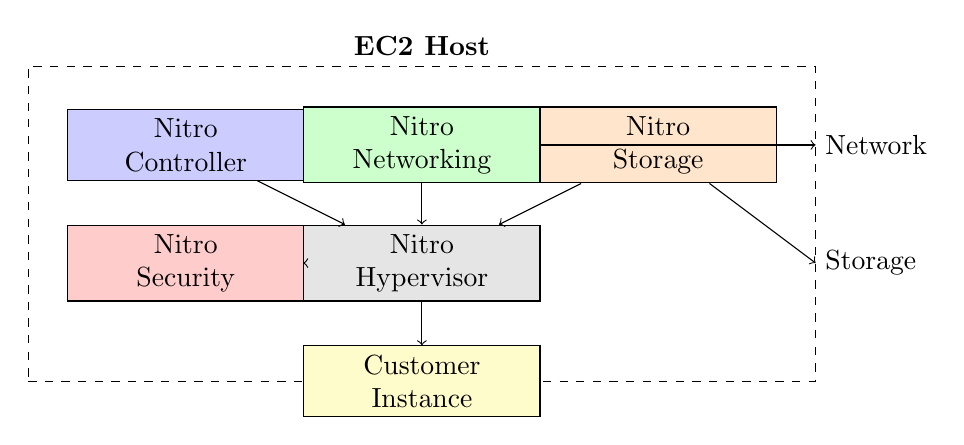
\begin{tikzpicture}[
    box/.style={rectangle, draw, minimum width=3cm, minimum height=0.8cm, align=center},
    bigbox/.style={rectangle, draw, dashed, minimum width=10cm, minimum height=4cm}
]
% EC2 Host
\node[bigbox] (host) at (0,0) {};
\node[above] at (host.north) {\textbf{EC2 Host}};

% Nitro Cards
\node[box, fill=blue!20] (ctrl) at (-3,1) {Nitro\\Controller};
\node[box, fill=green!20] (net) at (0,1) {Nitro\\Networking};
\node[box, fill=orange!20] (stor) at (3,1) {Nitro\\Storage};
\node[box, fill=red!20] (sec) at (-3,-0.5) {Nitro\\Security};

% Hypervisor
\node[box, fill=gray!20] (hyp) at (0,-0.5) {Nitro\\Hypervisor};

% Instance
\node[box, fill=yellow!20] (inst) at (0,-2) {Customer\\Instance};

% Connections
\draw[->] (ctrl) -- (hyp);
\draw[->] (net) -- (hyp);
\draw[->] (stor) -- (hyp);
\draw[->] (sec) -- (hyp);
\draw[->] (hyp) -- (inst);

% External
\node[right] at (5,1) {Network};
\draw[->] (net) -- (5,1);
\node[right] at (5,-0.5) {Storage};
\draw[->] (stor) -- (5,-0.5);
\end{tikzpicture}
\caption{AWS Nitro系统架构}
\end{figure}

\subsection{网络性能优化机制}

\subsubsection{单流带宽规格}

AWS Nitro网络针对不同类型的流量提供差异化的带宽保证：

\begin{table}[htbp]
\centering
\caption{Nitro网络单流带宽规格}
\begin{tabular}{@{}lll@{}}
\toprule
\textbf{流类型} & \textbf{带宽} & \textbf{适用场景} \\
\midrule
外部/默认流 & 5 Gbps & 互联网、跨区域 \\
Cluster Placement Group & 10 Gbps (TCP) / 8 Gbps (UDP) & 同AZ物理邻近 \\
ENA Express & 25 Gbps & 同AZ内基于SRD \\
EFA & 最高3.2 Tbps & HPC/ML工作负载 \\
\bottomrule
\end{tabular}
\end{table}

\subsubsection{数据包处理加速路径}

Nitro Card实现了连接状态缓存机制：

\begin{enumerate}
    \item \textbf{首包处理}：完整的安全组、路由、ACL检查，建立连接状态
    \item \textbf{后续包处理}：直接查询缓存的连接状态，走加速路径
    \item \textbf{Conntrack缓存}：Nitro Card维护每个流的连接跟踪表
\end{enumerate}

首包由于需要建立状态，延迟较高；后续包通过状态缓存实现低延迟转发。

\section{SRD协议：可扩展可靠数据报}

\subsection{SRD设计哲学}

SRD (Scalable Reliable Datagram) 是AWS为数据中心网络设计的专有传输协议，其核心创新在于：

\begin{itemize}
    \item \textbf{可靠但乱序传输}：保证数据可靠到达，但不保证顺序
    \item \textbf{应用层排序}：将顺序控制交给应用层，避免队头阻塞
    \item \textbf{消息为中心}：提供消息级别的网络抽象
\end{itemize}

\subsection{SRD四大核心技术}

\begin{enumerate}
    \item \textbf{智能多路径传输}
    \begin{itemize}
        \item 单流分布在最多64条并行路径
        \item 充分利用Clos网络的多路径特性
        \item 自动检测和避让拥塞路径
    \end{itemize}
    
    \item \textbf{微秒级重传}
    \begin{itemize}
        \item Nitro Card硬件实现重传
        \item 重传延迟从毫秒级降至微秒级
        \item 亚毫秒级拥塞控制响应
    \end{itemize}
    
    \item \textbf{数据包级拥塞控制}
    \begin{itemize}
        \item 实时检测路径拥塞
        \item 动态迁移流量到空闲路径
        \item 避免热点和Incast问题
    \end{itemize}
    
    \item \textbf{硬件完全卸载}
    \begin{itemize}
        \item 所有SRD处理在Nitro Card完成
        \item 不占用主机CPU资源
        \item 透明支持TCP/UDP应用
    \end{itemize}
\end{enumerate}

\subsection{SRD vs 传统协议对比}

\begin{table}[htbp]
\centering
\caption{传输协议技术对比}
\begin{tabular}{@{}lcccc@{}}
\toprule
\textbf{协议} & \textbf{可靠性} & \textbf{多路径} & \textbf{延迟} & \textbf{部署复杂度} \\
\midrule
TCP & 可靠有序 & 单路径 & 毫秒级 & 软件实现 \\
UDP & 无保证 & 应用决定 & 微秒级 & 简单 \\
InfiniBand RC & 可靠有序 & 硬件多路径 & 微秒级 & 需专用HCA \\
RoCE v2 & 依赖网络层 & 硬件多路径 & 微秒级 & 需无损以太网 \\
\textbf{SRD} & \textbf{可靠乱序} & \textbf{64路径} & \textbf{微秒级} & \textbf{需Nitro} \\
Falcon & 可靠传输 & 硬件多路径 & 微秒级 & 需Intel IPU \\
\bottomrule
\end{tabular}
\end{table}

\subsection{SRD三大应用场景}

\subsubsection{场景1: EFA (HPC/ML专用加速)}

EFA (Elastic Fabric Adapter)是SRD技术的首个主要战场：

\textbf{HPC应用性能}：
\begin{itemize}
    \item 计算流体动力学(CFD)：扩展到数千核心，性能媲美InfiniBand集群
    \item 天气预报模型：支持更细网格、更精确预报
    \item 基因组计算：显著减少序列比对和组装时间
\end{itemize}

\textbf{ML训练改进}：
\begin{itemize}
    \item 端点延迟降低30\%
    \item 小消息Allreduce性能提升50\%
    \item PyTorch FSDP训练性能提升18\%
    \item Megatron-LM性能提升8\%
\end{itemize}

\subsubsection{场景2: EBS io2 Block Express (存储加速)}

SRD集成到EBS最高性能卷类型：
\begin{itemize}
    \item 延迟改善：2.5-3.5倍降低
    \item 一致性亚毫秒I/O响应
    \item 客户案例：SQL查询时间减少30\%，TPS提升20\%
\end{itemize}

\subsubsection{场景3: ENA Express (通用网络加速)}

2022年发布的ENA Express实现了SRD技术的民主化：

\textbf{透明性特征}：
\begin{itemize}
    \item 无需修改应用代码
    \item 无需安装特殊驱动
    \item API/控制台一键开启
    \item 所有TCP/UDP自动走SRD
\end{itemize}

\textbf{性能提升}：
\begin{itemize}
    \item P99.9延迟降低85\%
    \item 单TCP流带宽：5 Gbps $\rightarrow$ 25 Gbps
\end{itemize}

\textbf{适用工作负载}：文件系统、内存数据库、媒体编码、大数据分析、微服务架构

\section{EFA演进与AI基础设施}

\subsection{EFA三代演进}

\begin{table}[htbp]
\centering
\caption{EFA架构演进}
\begin{tabular}{@{}llll@{}}
\toprule
\textbf{版本} & \textbf{年份} & \textbf{带宽} & \textbf{关键特性} \\
\midrule
EFA v1 & 2018 & 100 Gbps & OS bypass, MPI/NCCL支持 \\
EFA v2 & 2022 & 200 Gbps & 延迟降低30\% \\
EFA v3 & 2024 & 3.2 Tbps & H200 GPU, 延迟降低35\% \\
\bottomrule
\end{tabular}
\end{table}

\subsection{EFA-only接口 (2024年10月)}

\textbf{背景问题}：
\begin{itemize}
    \item 传统EFA耦合ENA设备，消耗IP地址
    \item AI/ML规模扩大时IPv4地址空间受限
    \item Linux多接口路由挑战（源IP不匹配）
\end{itemize}

\textbf{解决方案}：
\begin{itemize}
    \item EFA-only接口：仅EFA设备，无ENA设备
    \item 使用SRD协议通过MAC地址通信
    \item 不分配IP地址，解决扩展性问题
\end{itemize}

\textbf{使用限制}：
\begin{itemize}
    \item 只能作为辅助接口
    \item 主接口必须是EFA+ENA或纯ENA（用于TCP/IP路由）
\end{itemize}

\subsection{Trainium芯片与UltraServers}

\subsubsection{Trainium2技术规格}

\begin{table}[htbp]
\centering
\caption{Trainium2与Trn2实例规格}
\begin{tabular}{@{}ll@{}}
\toprule
\textbf{组件} & \textbf{规格} \\
\midrule
单芯片算力 & 万亿次计算/秒 \\
单芯片内存 & 96GB HBM3e \\
单芯片引擎 & 8×NeuronCore-V3 \\
Trn2芯片数 & 16个Trainium2 \\
Trn2算力 & 20.8 FP8 petaflops \\
Trn2内存 & 1.5TB HBM，46TB/s带宽 \\
Trn2网络 & 3.2Tbps EFA \\
价格性能 & 比GPU实例好30-40\% \\
\bottomrule
\end{tabular}
\end{table}

\subsubsection{Trn2 UltraServers}

UltraServers是AWS为超大规模模型训练推出的全新EC2产品：

\begin{itemize}
    \item \textbf{架构}：4个Trn2服务器合并为一个单元
    \item \textbf{芯片}：64个Trainium2芯片
    \item \textbf{互联}：NeuronLink超高速互连（蓝色线缆标识）
    \item \textbf{算力}：83.2 FP8 petaflops
    \item \textbf{内存}：6TB HBM，185TB/s总带宽
    \item \textbf{网络}：12.8Tbps EFA
\end{itemize}

\textbf{优势}：
\begin{itemize}
    \item 推理：业界领先的响应时间，最佳实时体验
    \item 训练：更快的集体通信，提升模型并行效率
\end{itemize}

\subsubsection{Project Rainier}

AWS与Anthropic合作打造的超大规模AI训练集群：

\begin{itemize}
    \item \textbf{规模}：近50万Trainium2芯片
    \item \textbf{部署}：跨多个美国数据中心
    \item \textbf{时间}：2024年12月宣布，12个月内完成部署
    \item \textbf{扩展}：预计2025年底达100万+芯片
    \item \textbf{算力}：为Anthropic提供比之前多5倍的训练算力
\end{itemize}

\subsubsection{Trainium3 (2025年底)}

AWS下一代AI芯片：

\begin{itemize}
    \item \textbf{工艺}：3nm（AWS首个3nm芯片）
    \item \textbf{算力}：2.52 PFLOPS FP8/芯片
    \item \textbf{内存}：144GB HBM3e（比Trainium2多1.5倍）
    \item \textbf{带宽}：4.9TB/s（高1.7倍）
    \item \textbf{UltraServer}：144芯片，362 FP8 PFLOPS
    \item \textbf{性能}：比Trn2 UltraServer高4.4倍
    \item \textbf{能效}：提升4倍以上
\end{itemize}

\section{云厂商网络架构对比}

\subsection{L1-L7技术栈对比}

\begin{table}[htbp]
\centering
\caption{云厂商数据中心网络技术栈对比}
\begin{tabular}{@{}lccc@{}}
\toprule
\textbf{OSI层} & \textbf{AWS} & \textbf{Google Cloud} & \textbf{Azure} \\
\midrule
L7应用 & EFA API & Cloud RDMA API & IB Verbs API \\
L6表示 & Nitro编码 & ALTS加密 & Azure Boost编码 \\
L5会话 & Nitro会话 & gRPC RPC & MANA会话 \\
\textbf{L4传输} & \textbf{SRD} & \textbf{Falcon} & \textbf{RoCE v2/IB} \\
L3网络 & VPC+ENA Express & Andromeda 2.1 & AccelNet/MANA \\
L2链路 & 以太网 & 以太网 & 以太网/IB \\
L1物理 & QSFP-DD+PAM4 & 光纤+OCS & 光纤+PAM4/HCF \\
\textbf{硬件} & \textbf{Nitro v5 DPU} & \textbf{Intel IPU E2000} & \textbf{Azure Boost} \\
\bottomrule
\end{tabular}
\end{table}

\subsection{技术路线差异}

\begin{itemize}
    \item \textbf{AWS}：专有SRD协议 + 标准以太网 + Nitro DPU硬件卸载
    \item \textbf{Google Cloud}：专有Falcon协议 + Intel IPU + OCS光电路交换
    \item \textbf{Microsoft Azure}：RoCE v2/InfiniBand混合 + Azure Boost + MANA
\end{itemize}

三种路线各有优势，AWS的SRD方案在标准以太网基础设施上实现了类似InfiniBand的低延迟高性能，同时保持了与TCP/IP应用的兼容性。


\subsection{多云互联与网络开放趋势}

\subsubsection{AWS-Google Cloud网络合作 (2025年)}

2025年11月，AWS和Google Cloud宣布联合工程合作，简化多云网络：

\begin{itemize}
    \item 结合AWS Interconnect - multicloud和Google Cross-Cloud Interconnect
    \item 几分钟内配置云间私有加密连接（vs 传统数周）
    \item MACsec强制加密和四重冗余
    \item 开放规范，其他提供商可采用
    \item Microsoft Azure计划2026年加入
\end{itemize}

\subsubsection{Oracle-Google Cloud合作伙伴关系 (2024年)}

2024年6月，Oracle和Google Cloud宣布战略合作：

\begin{itemize}
    \item \textbf{Oracle Database@Google Cloud}：OCI数据库服务运行在Google数据中心
    \item 首批区域：美国东部（阿什本）、美国西部（盐湖城）、英国南部（伦敦）、德国中部（法兰克福）
    \item 无跨云数据传输费用
    \item 直接在Google Cloud中运行Oracle Exadata和Autonomous Database
\end{itemize}

% ============================================================
\section{洛神：阿里云软硬一体化网络的工程实践}
% ============================================================

前面的章节我们讨论了DPU和SmartNIC作为数据中心"第三支柱"的理论基础。现在，让我们走进阿里云洛神系统的工程实践，看看这些理念是如何在真实的超大规模云网络中落地的。

2018年的一个深夜，阿里云网络团队的工程师们盯着监控大屏上不断攀升的CPU利用率曲线，心情沉重。随着集团上云战略的推进，网络流量呈数量级增长，基于x86+DPDK的软件转发方案已经触及性能天花板。单个CPU核心被打爆的情况越来越频繁，这意味着：\textbf{软件转发的时代即将结束，软硬一体化的时代必须到来。}

这就是洛神2.0软硬一体化高性能网络项目的起点。

% ============================================================
\subsection{NFV平台的困境与洛神的诞生}
% ============================================================

\subsubsection{从电信行业的NFV说起}

网络功能虚拟化（NFV, Network Functions Virtualization）的概念最早由欧洲电信标准协会（ETSI）提出。运营商们厌倦了笨重昂贵的专用网络设备，希望用标准的IT虚拟化技术来承载DNS、NAT、防火墙等网络功能。

NFV的核心理念是\textbf{软硬件解耦}：让传统网络功能不再依赖专用硬件，而是运行在通用x86服务器或容器上，从而获得资源灵活共享、快速部署、弹性伸缩等云原生特性。

在阿里云洛神1.0架构中，云虚拟网络的网元（XGW、NAT网关、SLB、边界路由器等）正是以NFV的理念部署的——基于通用x86物理机，配合DPDK做软转发。单台物理机可以提供160Gbps/26Mpps的转发能力，在当时已经算是不错的成绩。

\subsubsection{物理机部署的四大痛点}

然而，随着互联网流量的快速增长和集团上云的全面推进，物理机形态的网络设备暴露出越来越严重的问题。让我们逐一分析这些痛点背后的深层原因。

\textbf{痛点一：采购和部署周期长}

假设阿里云需要在一个新Region上线NAT网关功能。如果采用物理机部署，从需求提出到最终上线，需要经历：硬件选型→供应商谈判→下单采购→工厂生产→物流运输→机房上架→系统部署→测试验收。这个流程通常需要数周甚至数月时间。

在云时代，客户的需求是随时变化的。一个创业公司今天可能只需要10Mbps的带宽，明天就可能因为产品爆红需要1Gbps。物理机的长交付周期与云服务的即时性需求形成了根本矛盾。

\textbf{痛点二：缺乏弹性}

双十一的流量是日常的10倍以上。如果按峰值采购物理机，平时的利用率将极低，造成巨大浪费；如果按均值采购，大促时必然崩溃。这种\textbf{削峰填谷}的难题在物理机架构下几乎无解。

更严重的是，某些业务的流量模式完全不可预测。一个网红直播可能在几分钟内带来百倍流量激增，物理机集群根本无法及时响应。

\textbf{痛点三：故障影响面广}

传统物理机采用集中化部署，一台设备可能承载数千个租户的网络流量。一旦这台设备发生故障，影响的不是某个单一客户，而是数千个客户的业务。这种\textbf{单点故障的爆炸半径}在云环境下是不可接受的。

\textbf{痛点四：迭代缓慢}

新特性发布需要经历：开发→测试→灰度→全量上线。在物理机架构下，每个环节都涉及物理设备的操作，发布周期以月为单位。而在互联网竞争中，\textbf{速度就是生命}。竞争对手可能在一周内上线新功能，而你的物理机架构需要三个月——这意味着你已经输了。

这四个痛点本质上都是\textbf{物理机的刚性}与\textbf{云服务的弹性}之间的矛盾。要解决这个问题，必须让网络功能本身也成为云上的弹性服务。

\subsubsection{洛神2.0的破局思路}

面对这些挑战，阿里云网络团队在洛神2.0架构中做出了关键决策：

\begin{quote}
\textbf{除了VPC（AVS、XGW）和ALB等基础网络功能外，其他网元（NAT网关、VPN、PrivateLink、TR等）全部基于NFV平台进行开发，以ECS/Docker为部署形态，对用户提供商原生网络服务。}
\end{quote}

这个决策的本质是\textbf{用云的能力来增强云网络}——让网络功能本身也成为云上的弹性服务，而不是固定在物理机上的静态功能。

NFV平台按照ETSI MANO模型，划分为三大核心模块：

\begin{itemize}
    \item \textbf{VIM（虚拟基础设施管理器）}：管理虚拟计算、存储、网络资源的生命周期，包括创建、删除、健康检查、故障自动隔离和恢复
    \item \textbf{VNFM（虚拟网络功能管理器）}：为业务网元分配逻辑计算资源，实现"一虚多"（单ECS虚拟成多个VNF Member）和"多虚一"（多VNF Member组成逻辑Group）
    \item \textbf{NFVO（网络功能虚拟化编排器）}：实现分布式的快慢速转发架构，首包由慢速路径处理，后续报文走硬件快速路径
\end{itemize}

\subsubsection{Shuffle Sharding：控制爆炸半径}

NFV平台采用了一种名为\textbf{Shuffle Sharding}的技术来实现高可用和故障隔离。其核心思想是：

\begin{itemize}
    \item 以VNF Group粒度为网元提供计算资源服务
    \item 单个计算资源可以在多个VNF Group间共享
    \item 同一个VNF Group的逻辑计算资源尽量打散在不同物理机，防止单机故障影响租户
    \item 不同VNF Group的计算资源不完全重叠，防止租户间相互影响
\end{itemize}

这种设计将故障的"爆炸半径"控制在最小范围内。即使某个计算节点发生故障，也只会影响少数几个VNF Group，而不会波及整个Region的所有租户。

% ============================================================
\subsection{洛神2.0软硬一体化架构全解}
% ============================================================

2021年2月23日，洛神2.0全面落地庆功会在阿里云EFC园区隆重举行。经过3年的努力，软硬一体化项目取得了阶段性成果：云网络的三大基础组件（AVS/XGW/Ali-LB）实现了全面软硬一体化，性能和稳定性得到大幅提升。

\subsubsection{从Kernel到DPDK：第一次性能飞跃}

阿里云网络的演进经历了三个阶段：

\begin{enumerate}
    \item \textbf{Kernel转发时代}：早期基于Linux内核协议栈，性能约1Mpps
    \item \textbf{DPDK时代}：5-6年前全面演进至DPDK转发，性能提升4-5倍，稳定性大幅提升
    \item \textbf{软硬一体化时代}：从DPDK到可编程硬件，性能再提升一个数量级
\end{enumerate}

DPDK无疑是成功的，但随着技术和业务的发展，它面临新的挑战：

\begin{itemize}
    \item \textbf{技术挑战}：ECS网络速率从25G→50G→100G，每2-3年翻一番；但摩尔定律放缓，CPU核数提升变慢，单核性能瓶颈无解
    \item \textbf{业务挑战}：集团上云带来数十Tbps的大流量，IoT和NAS带来数十Gbps的大单流，压测和攻击带来突发流量
\end{itemize}

\subsubsection{软硬一体化的技术选型}

软转发不行就上硬件，这是合理且自然的演进。但云网络的业务高度定制化，无法使用转发行为固化的传统硬件，需要\textbf{可编程硬件}来满足业务定制化和需求持续迭代。

在选择硬件加速方案时，团队需要回答一个关键问题：\textbf{有状态业务和无状态业务应该如何选择？}

\textbf{有状态业务}（如AVS的Session表、Ali-LB的连接状态）需要存储大量状态数据。以AVS为例，一台物理机上可能运行数百个虚拟机，每个虚拟机有数千个并发连接，Session表项可能达到百万级别。可编程交换芯片的片内SRAM容量有限（如Tofino单pipeline仅120MB），无法容纳如此大量的状态数据。因此需要\textbf{FPGA+片外DDR}的方案，通过外部存储扩展来支撑大规模状态表。

\textbf{无状态业务}（如XGW的路由表查找、IGW的ACL匹配）只需要查找转发表，不需要维护连接状态。这类业务的特点是：表项相对固定、查找逻辑简单、流量巨大。可编程交换芯片（如Tofino）具有极高的转发性能（3.2Tbps）和极低的成本，是这类业务的理想选择。

基于以上分析，团队做出了如下技术选型：

\begin{table}[htbp]
\centering
\caption{洛神2.0软硬一体化技术选型对比}
\begin{tabular}{|l|l|l|l|}
\hline
\textbf{业务类型} & \textbf{硬件方案} & \textbf{代表产品} & \textbf{特点} \\
\hline
有状态业务 & FPGA+DDR & AVS、Ali-LB & Session/Flow数量大，需片外DDR扩展 \\
\hline
无状态业务 & 可编程交换芯片 & XGW、CGW、IGW & 性能高、成本低、投资收益比最大化 \\
\hline
\end{tabular}
\end{table}

\subsubsection{AVS硬件加速：从5Mpps到28Mpps}

AVS（Apsara Virtual Switch）硬件加速项目于2018年7月启动，2019年7月灰度上线，2020年3月批量上线。经过近3年的努力，支持AVS硬件加速的MoC2.0已在集团和公共云大规模上线。

通过Fastpath硬件加速，AVS转发性能\textbf{从5Mpps飞跃到28Mpps}，提升约5倍，转发延时下降50\%。这个性能大幅领先AWS、华为、腾讯等友商。在需要增强型网络的应用场景，Fastpath的30Mpps对比软转节省十几个CPU核心，成本大幅下降。

\subsubsection{Ali-LB硬件加速：解决单核打爆难题}

作为流量汇聚点，Ali-LB面临的性能和稳定性压力比AVS更大。2020年7月项目启动，经过近9个月的努力达到灰度状态。

通过Fastpath硬件加速：
\begin{itemize}
    \item bps性能提升5倍
    \item pps性能提升8倍
    \item 可轻松支持DFS大流量和NAS大单流
    \item 彻底解决CPU单核打爆问题
\end{itemize}

Ali-LB采用单卡2×100G配置，使用2路并行的Fastpath提升性能。兼容标准网卡功能，支持RSS/FlowDir和CSO，数据和配置通道通过AliDMA实现高性能多队列DMA。

% ============================================================
\subsection{硬件公网网关igw-sna：从软件到芯片的跃迁}
% ============================================================

\subsubsection{背景：x86架构的瓶颈}

公网网关（IGW）是云网络的流量出入口，承载着VPC到公网的所有流量。早期基于x86+DPDK架构实现，但随着业务复杂度和流量的增长，面临严重的性能和稳定性问题。

一个典型的场景是NAT网关+带宽包场景：为了给200M带宽包进行精确限速，需要将所有流量汇聚到1台xgw的1个core上进行限速处理。这种流量汇聚加重了xgw负担，容易打爆CPU，引入稳定性风险。

\subsubsection{SNA平台：可编程交换芯片的威力}

为了解决x86的问题，阿里云引入了\textbf{igw-sna}方案，基于自研的SNA（Smart Network Appliance）平台实现。

SNA底层芯片采用\textbf{Barefoot Tofino}芯片，具有以下规格：
\begin{itemize}
    \item 4个pipeline
    \item 32个100G端口
    \item 支持3.2T流量转发
    \item 单个pipeline只有120MB SRAM、6MB TCAM
\end{itemize}

资源非常紧张，因此需要一系列优化手段来最大化利用硬件资源。

\subsubsection{配置的水平分割}

为了解决硬件资源不足问题，igw-sna采用了\textbf{配置水平分割}策略：

\begin{itemize}
    \item \textbf{拆分前}：单AZone承载全Region业务配置，无法水平扩展
    \item \textbf{拆分后}：通过集群水平扩展承载全Region业务配置
\end{itemize}

拆分带来的好处：
\begin{enumerate}
    \item 优化配置下发时间
    \item 缩短故障恢复时间
    \item 支持更大规模的EIP和带宽包
\end{enumerate}

\subsubsection{Pipeline折叠：榨干芯片资源}

Tofino芯片具有4个pipeline，其中2个是external pipeline（连接外部以太网口），2个是internal pipeline。为了充分利用硬件资源，采用了\textbf{pipeline折叠}设计，将internal资源也充分利用。

更进一步，如果配置非对称下发，存储规格能够提升1倍。这种设计让igw-sna能够在有限的硬件资源下支持更多的业务表项。

\subsubsection{业务下沉与Fallback机制}

对于NAT网关这类有状态业务，如果在硬件存储session状态需要占用较多资源，Tofino芯片当前规格无法支持。因此采用了\textbf{业务下沉}策略：

\begin{itemize}
    \item 短期NAT1.0业务fallback给xgw-x86处理
    \item IGW-SNA上只做限速处理，不做业务处理
    \item 非共享带宽包的EIP限速下沉到AVS
\end{itemize}

这种设计让igw-sna能够专注于它最擅长的无状态高速转发，将复杂的有状态处理留给软件。

\subsubsection{灰度与故障逃逸}

作为全新架构，igw-sna引入了灵活的业务AZone拆分：将EIP路由宣告AZone和EIP业务处理AZone分离。

这种设计的好处：
\begin{enumerate}
    \item 可以灵活引流到sna进行灰度
    \item 出现问题时可通过快速业务切换逃逸，避免复杂的路由切换
    \item 通过表项对账提前暴露配置不一致问题
\end{enumerate}

目前igw-sna已在北上杭深上线，承载着95\%+的公网业务流量，线上CPU打高告警得到显著收敛。

% ============================================================
\subsection{SIGCOMM 2021论文解读：洛神的学术贡献}
% ============================================================

2021年，阿里云网络团队的论文《Sailfish: Accelerating Cloud-Scale Multi-Tenant Multi-Service Gateways with Programmable Switches》被网络领域顶会SIGCOMM录用。这是继SIGCOMM 2020《VTrace》之后，阿里云网络再次入选SIGCOMM的论文。

\subsubsection{论文背景：云网关的独特挑战}

阿里云作为国内领先的云服务提供商，其业务发展速度和数据增长规模日新月异。云网关作为数据中心各种流量的汇聚点，承载的压力前所未有。

相比传统流量转发设备，云网关具备以下特点：
\begin{itemize}
    \item \textbf{高吞吐、低时延}：从早期内核转发（1Mpps）到DPDK（几Mpps）到硬件卸载（几十Mpps）
    \item \textbf{表项规模大}：一个大型Region的路由表是十万量级，VM-NC是百万量级
    \item \textbf{表项种类多}：要满足租户内VM互访、不同租户VPC打通、云上VM访问公网、IDC上云和下云、跨域云设备之间的访问
\end{itemize}

\subsubsection{核心洞察：数据中心的2/8定律}

从阿里云数据中心多年的流量统计来看，流量基本符合\textbf{2/8定律}：20\%的表项承载了80\%的流量。

基于这个洞察，论文提出了系列解决方案：
\begin{enumerate}
    \item 从流量2/8定律出发，做软硬件协同
    \item 有别于x86在计算资源上做全量scale-out，在存储上做水平分割的scale-out
    \item 单机优化：流水线折叠、表项哈希分流、表项复用、资源池化
\end{enumerate}

\subsubsection{软硬件协同架构}

XGW-H作为流量主要出入口，XGW-x86为辅：
\begin{itemize}
    \item 高转发性能、大吞吐量的XGW-H为默认网关
    \item XGW-H存储表项少、流量大的业务，同时作为XGW-x86的导流器
    \item XGW-x86负责占用表项空间大、业务逻辑复杂但流量占比小的业务
\end{itemize}

\subsubsection{表项水平分割}

采用多个集群承担Region内所有表项，单集群承担部分用户表项。物理网络的负载均衡交换机根据数据包VNI将其分配给相应的网关集群。

好处：
\begin{enumerate}
    \item 提高可扩展性：新增集群就能容纳更多用户
    \item 限制故障影响范围
    \item 降低表项处理和下发时间
\end{enumerate}

\subsubsection{惊人的性能提升}

经过多轮优化，新的Sailfish XGW-H取得了显著成果：
\begin{itemize}
    \item 延时降低\textbf{95\%}
    \item bps提升\textbf{20倍}
    \item pps提升\textbf{71倍}
\end{itemize}

IPv6优化方面，75\% IPv4表项、25\% IPv6表项场景下，SRAM压缩了30\%，TCAM压缩了94\%。

% ============================================================
\subsection{智能网卡与Overlay网络：卸载的边界在哪里}
% ============================================================

\subsubsection{云计算网络的四大挑战}

在深入了解Overlay网络之前，我们先看看云计算数据中心面临的网络问题：

\begin{enumerate}
    \item \textbf{大容量MAC/ARP表项}：5000台服务器按1:20虚拟化，就有10万个虚拟机，需要20万个MAC地址。主流接入交换机只有32K MAC表项，无法满足需求。
    
    \item \textbf{4K VLAN Trunk问题}：静态配置VLAN trunk all会导致任一VLAN内的广播风暴影响全网所有VLAN。
    
    \item \textbf{4K VLAN上限问题}：租户及业务规模超出VLAN上限（4K）时无法支撑客户需求。
    
    \item \textbf{虚拟机迁移网络依赖}：VM迁移需要在同一个二层域内，基于IP子网的区域划分限制了二层网络连通性规模。
\end{enumerate}

\subsubsection{Overlay网络技术原理}

Overlay网络技术是指在一种网络架构上叠加虚拟化技术的模式，对基础网络不进行大规模修改，实现应用在网络上的承载。

Overlay技术的核心特点：
\begin{itemize}
    \item 采用隧道技术实现L2oIP的封装
    \item 物理网络只看见Overlay边缘节点的MAC地址，MAC表项非常有限
    \item 提供24bits长度的隔离ID（VNI），最大支持16M租户
    \item 通过名址分离，内层IP地址完全作为寻址标签，不同subnet之间可以二层互通
\end{itemize}

\subsubsection{VXLAN：主流的Overlay协议}

VXLAN（Virtual eXtensible LAN）是当前最主流的Overlay标准，其优势在于：

\begin{enumerate}
    \item \textbf{标准化程度高}：Cisco/VMware/Citrix/RedHat/Broadcom等主流厂商支持
    \item \textbf{负载均衡友好}：利用UDP源端口号进行ECMP，传统网络设备即可支持
    \item \textbf{成熟度高}：基于通用的UDP传输，在ESXi和Open vSwitch、主流网络芯片已经实现
\end{enumerate}

\begin{table}[htbp]
\centering
\caption{主流Overlay技术对比}
\begin{tabular}{|l|l|l|l|l|}
\hline
\textbf{特性} & \textbf{VXLAN} & \textbf{NVGRE} & \textbf{STT} & \textbf{Geneve} \\
\hline
封装方式 & MAC in UDP & MAC in GRE & MAC in TCP & MAC in UDP \\
\hline
VN Context & 24位VNI & 24位VSID & 64位Context ID & 24位VNI \\
\hline
ECMP支持 & 源端口号 & Flow ID & 源端口号 & 源端口号 \\
\hline
标准化 & 成熟 & 微软主推 & VMware私有 & 工作组草案 \\
\hline
\end{tabular}
\end{table}

\subsubsection{智能网卡上的Overlay卸载}

Overlay网络虽然解决了虚拟化网络的扩展性问题，但隧道封装/解封装带来了额外的CPU开销。智能网卡（SmartNIC）可以将这些开销从主机CPU卸载。

Overlay在智能网卡上的实现有两种形态：
\begin{itemize}
    \item \textbf{硬件VTEP}：网络设备执行封装解封装，支持虚机与非虚拟化服务器的混合组网
    \item \textbf{软件VTEP}：驻留在虚拟机管理程序主机中，直接支持虚拟化工作负载
\end{itemize}

阿里云MoC（Mellanox ConnectX）智能网卡就支持硬件VXLAN offload，可以将封装解封装、校验和计算等工作从主机CPU完全卸载。

% ============================================================
\subsection{可编程硬件四层负载均衡：LVS的硬件化之路}
% ============================================================

\subsubsection{背景：软件负载均衡的困境}

阿里集团为业务方提供了基于L4的网络负载均衡服务。但在大促等业务场景下，出现了新的挑战：

\begin{itemize}
    \item "负载均衡"集群之间因为业务发展不均衡，出现热点流量，导致负载均衡自身"不均衡"
    \item 大数据业务场景下，经常出现大象流导致单核CPU 100\%，进而导致业务部分超时
\end{itemize}

\subsubsection{Smart-X：两级流量均衡架构}

阿里云网络团队开发了\textbf{Smart-X}两级负载均衡系统，由以下组件构成：

\begin{enumerate}
    \item \textbf{Smart-GW}：第一级流量调度集群，负责虚拟业务（VIP）的发布和调度业务流量到第二级集群。采用硬件转发技术、不做业务处理、不保持业务状态，单集群可达12.8Tb/s处理能力。
    
    \item \textbf{Smart-LB}：第二级集群，负责虚拟业务的实际调度到后台服务器。与虚拟服务解耦，调度什么业务流量完全取决于Smart-GW的动态调度。
    
    \item \textbf{Smart-Alive}：基于服务器的健康检查集群，负责后台服务器状态的监控并通知Smart-LB集群。
    
    \item \textbf{智能调度系统}：管理监控所有集群，根据负载情况动态调整Smart-GW到Smart-LB的虚拟服务级别调度。
\end{enumerate}

\subsubsection{性能对比：10倍的提升}

在ODPS场景的落地结果表明：
\begin{itemize}
    \item 利用可编程网络硬件的负载均衡可以比软件负载均衡LVS提升\textbf{10倍}的性能
    \item 单VIP超过Tb/s流量能力
    \item 负载均衡集群之间负载值（CPU、session等）差距在\textbf{5\%}以内
    \item 完全避免单核流量打爆的问题
\end{itemize}

\subsubsection{资源池化：让大促成为常态}

传统负载均衡方案的问题是不同虚拟业务独占资源，集群利用率不高。Smart-X的两级调度架构让第二级Smart-LB可以互相共享资源——一个Smart-GW集群可以连接最多256个Smart-LB集群，组成一个巨大的虚拟服务调度池。

这意味着：\textbf{随着二级集群池容量的不断增加，即使大促增加的流量也能在整个系统内消化，根本不需要为大促进行扩容或者进行人工的流量调度。}

% ============================================================
\subsection{可编程硬件在阿里的全景应用}
% ============================================================

\subsubsection{云豹与Griffin：可编程软件平台}

可编程芯片技术和整个技术开发生态还不够成熟，市场上没有一个软件开发平台来支持可编程应用的开发。阿里云AIS可编程团队在2017年底就提出了可编程软件平台的概念。

\textbf{云豹}可编程软件平台（第一代）于2018年3月推出，一直支撑着Smart-X和XGW产品的开发。

\textbf{Griffin}平台（第二代）于2018年7月提出概念，是一个集成可编程技术、AliNOS自研交换机和Netframe等功能的可编程软件平台，支持第三方从2层到7层全协议栈应用的开发。

\subsubsection{可编程硬件产品矩阵}

基于可编程硬件技术，阿里云已经落地了多款产品：

\begin{table}[htbp]
\centering
\caption{阿里云可编程硬件产品矩阵}
\begin{tabular}{|l|l|l|l|}
\hline
\textbf{产品} & \textbf{硬件基础} & \textbf{应用场景} & \textbf{性能指标} \\
\hline
Smart-X & Tofino可编程芯片 & 四级负载均衡 & 单集群12.8Tbps \\
\hline
XGW 2.0 & Tofino可编程芯片 & VPC网关 & 单机3.2Tbps \\
\hline
CGW-H & SNA平台 & 专线网关 & bps提升20倍 \\
\hline
IGW-H & SNA平台 & 公网网关 & pps提升80倍 \\
\hline
硬件Smart-NAT & SNA平台 & NAT网关 & 千万级session \\
\hline
硬件IDS & SNA平台 & 入侵检测 & 实时流量分析 \\
\hline
\end{tabular}
\end{table}

\subsubsection{双十一的实战检验}

2019年双十一，基于可编程交换芯片+P4的XGW 2.0承担了上云的绝大部分流量，在流量暴增的情况下稳如磐石。

2020年双十一，多个基于可编程芯片技术的产品支撑大促业务，总业务流量接近\textbf{30Tb/s}。

阿里云是\textbf{第一家}将可编程芯片技术产品化并规模商用化的公司，也是业界第一个将可编程技术在复杂应用场景（支持session）商用化的公司。

% ============================================================
\subsection{Azure Bluebird：微软裸金属SDN的另一条路}
% ============================================================

\subsubsection{论文背景}

Bluebird是微软和Intel合作，基于可编程ASIC实现的用于支持裸金属实例的高性能SDN转发平台，论文发表于NSDI 2022。与智能网卡（DPU）厂商（如Pensando）采用的在NIC上支持P4不同，微软是把Tofino搬到了ToR（Top of Rack）交换机上。

\subsubsection{为什么选择ToR而不是SmartNIC？}

微软在论文中解释了原因：
\begin{quote}
While smartNICs have proven to be effective overall, they are not a good fit for the bare-metal model given the integration requirements. This is mostly due to the complexities that would be introduced at the hypervisor and network stack of the host.
\end{quote}

主要原因：
\begin{enumerate}
    \item 会在hypervisor和host侧引入复杂性
    \item SDN stack的实现需要和特定的裸金属解耦，保证架构的通用性
\end{enumerate}

这种裸金属形态更接近托管物理机，各种配置都有，不是云厂商提供的统一形态，因此不适合直接采用SmartNIC。

\subsubsection{Bluebird架构设计}

Bluebird主要完成两个功能：
\begin{itemize}
    \item 租户隔离：每个租户绑定一个VRF（Virtual Routing and Forwarding）
    \item CA-to-PA映射：用户虚拟机地址到物理机地址的转换
\end{itemize}

Azure同样采用VXLAN overlay，使用VNI实现租户隔离。ToR上的每个接口都有一个关联的VRF，配置有报文转发给用户VM的路由。

\subsubsection{Route Cache：缓解硬件资源压力}

Bluebird面临和阿里云类似的问题：可编程芯片资源有限。Bluebird采用了\textbf{Route Cache}方案：

\begin{itemize}
    \item 根据用户对CA-PA条目的使用统计，让热点频繁使用的条目下发在硬件上
    \item 其他条目保留在软件内存（类似大象流卸载思想）
    \item 开发了基于DPDK的Software Forwarding Engine (SFE)，性能达200Kpps
    \item 硬件采用LRU算法进行条目置换
\end{itemize}

这种设计将原有规格增加了5倍。软件延时比硬件多8us，因此及时准确地将软件命中的CA-PA下发到硬件对性能十分关键。

\subsubsection{与洛神方案的对比}

\begin{table}[htbp]
\centering
\caption{Azure Bluebird与阿里云洛神方案对比}
\begin{tabular}{|l|l|l|}
\hline
\textbf{维度} & \textbf{Azure Bluebird} & \textbf{阿里云洛神} \\
\hline
硬件位置 & ToR交换机 & 专用网关设备/SmartNIC \\
\hline
适用场景 & 托管裸金属 & 公有云VM/裸金属 \\
\hline
功能范围 & 仅VNET（基础路由） & 完整VPC功能 \\
\hline
资源优化 & Route Cache & 表项水平分割+Pipeline折叠 \\
\hline
控制面 & 独立Bluebird Service & 分布式控制器 \\
\hline
\end{tabular}
\end{table}

\subsubsection{两种路线的深层分析}

微软选择ToR而非SmartNIC，本质上是一个\textbf{边界划分}的问题。对于托管裸金属场景，客户拥有完全的控制权，云厂商无法在主机内部署任何软件或硬件。ToR作为网络边界设备，是云厂商唯一能够控制的点。这种选择是\textbf{场景约束下的最优解}，而非技术优劣的判断。

相比之下，阿里云洛神面向的是公有云场景，云厂商拥有完整的控制权。SmartNIC可以直接部署在每台服务器上，将网络功能下沉到最靠近业务的位置，减少网络跳数，降低延迟。这是\textbf{公有云场景下的最优解}。

\textbf{资源优化策略的差异}也反映了两种场景的不同需求。Bluebird的Route Cache基于LRU算法，假设流量具有时间局部性——最近访问的CA-PA映射最可能被再次访问。这种设计适合相对稳定的业务流量。而洛神的表项水平分割+Pipeline折叠则是从\textbf{空间维度}解决问题，通过分布式部署和硬件资源最大化利用来支撑超大规模表项。

\textbf{对后续演进的影响}值得关注。微软的ToR路线意味着网络功能进一步向网络边缘集中，可能催生更强大的ToR交换机；而阿里的SmartNIC路线意味着网络功能进一步下沉到服务器，DPU可能成为每台服务器的标配。两条路线看似相反，实则殊途同归——\textbf{都在追求网络与计算的深度融合}。

Bluebird的关键启示：\textbf{ToR和NIC的边界正在变得模糊}。微软用ToR实现了部分SmartNIC的功能，而Google的Aquila（同年NSDI）则把ToR功能塞进NIC——虽然方式不同，但可以看出两种融合趋势。未来的数据中心网络架构，可能不再有明显的"网络设备"与"计算设备"之分，而是一个\textbf{网络与计算深度融合的统一基础设施}。

% ============================================================
\subsection{DPU架构的演进方向：从网卡到计算基础设施}
% ============================================================

\subsubsection{数据为中心的时代}

早在2016年，Intel就提出了\textbf{以数据为中心}的战略。过去以计算为中心的架构中，CPU和GPU速度远远快于网络，等待网络数据成了系统性能瓶颈。

随着网络速度的快速进步（10G→25G→100G→200G），CPU性能赶不上了，才出现了DPDK等软件加速方案。软件方案终究只是权宜之计，更多网络、存储、安全等特性必须卸载到硬件上完成才能达到最佳性能。

\subsubsection{DPU三要素}

2020年10月，英伟达CEO黄仁勋在GTC大会上发布了DPU（Data Processing Unit）产品路线图，称DPU将是未来数据中心计算的\textbf{三大支柱}之一：

\begin{quote}
``The CPU is for general purpose computing, the GPU is for accelerated computing and the DPU, which moves data around the data center, does data processing.''
\end{quote}

英伟达认为DPU必须具有三要素：
\begin{enumerate}
    \item 基于行业标准、高性能及软件可编程的多核CPU
    \item 高性能网络接口
    \item 灵活、可编程的加速引擎
\end{enumerate}

\subsubsection{主流DPU方案对比}

市场上推出DPU（或类似功能）的主要厂商可分为三类：

\begin{table}[htbp]
\centering
\caption{主流DPU方案对比}
\begin{tabular}{|l|l|l|l|}
\hline
\textbf{类型} & \textbf{代表厂商} & \textbf{特点} & \textbf{适用场景} \\
\hline
定制芯片 & Fungible、Pensando、AWS Nitro & 性能高、灵活性低 & 超大规模云厂商 \\
\hline
FPGA方案 & Intel、Xilinx & 灵活性高、成本高 & 需要快速迭代的场景 \\
\hline
通用CPU+加速器 & Nvidia/Mellanox Bluefield & 生态成熟、易编程 & 通用加速场景 \\
\hline
\end{tabular}
\end{table}

\subsubsection{演进趋势}

DPU的演进呈现以下趋势：
\begin{enumerate}
    \item \textbf{功能融合}：网络、存储、安全、虚拟化功能集成到单一芯片
    \item \textbf{计算卸载}：从单纯的数据搬运到在搬运中处理数据
    \item \textbf{软硬协同}：硬件加速与软件控制的紧密结合
    \item \textbf{生态成熟}：P4等可编程语言降低开发门槛
\end{enumerate}

% ============================================================
\subsection{xRDMA：RDMA产品化的工程挑战}
% ============================================================

\subsubsection{背景：内核协议栈的性能天花板}

如何不断提高网络性能，进一步提升业务性能，同时又能降低综合成本，是数据中心网络永恒的追求。

经过多年的发展，内核协议栈的性能优化逐渐接近天花板。让我们以一个具体的4KB数据发送为例，看看数据包在内核中经历了什么：

\begin{enumerate}
    \item \textbf{用户态到内核态切换}：应用程序调用send()，触发系统调用，CPU从用户态切换到内核态，保存上下文——约100ns开销
    
    \item \textbf{数据拷贝#1}：用户缓冲区数据拷贝到内核socket缓冲区——4KB数据约200ns
    
    \item \textbf{协议栈处理}：TCP分段、添加头部、计算校验和、拥塞控制逻辑——约500ns
    
    \item \textbf{数据拷贝#2}：内核socket缓冲区拷贝到网卡DMA缓冲区——约200ns
    
    \item \textbf{中断处理}：发送完成中断，CPU暂停当前工作处理中断——约1us
    
    \item \textbf{进程唤醒}：如果有数据到达，唤醒等待的进程，再次上下文切换——约100ns
\end{enumerate}

一次完整的发送-接收往返（ping-pong），数据需要经过\textbf{4次拷贝}，\textbf{2次上下文切换}，\textbf{2次中断处理}。对于4KB报文，这些开销累计可能达到\textbf{5-10微秒}。当网络延迟本身只有几微秒时，内核协议栈的开销成为了\textbf{不可忽视的瓶颈}。

更深层的问题在于：
\begin{itemize}
    \item \textbf{软件链路过长}：从socket API到网卡驱动，代码路径长达数千行，CPU流水线cache miss频繁
    \item \textbf{中断驱动模型}：每次报文到达都触发中断，高并发下中断风暴会拖垮系统
    \item \textbf{通用性代价}：内核协议栈需要兼容各种场景，大量通用性检查带来额外开销
\end{itemize}

这些开销在10G网络时代还可以接受，但在25G、100G网络时代，CPU已经无法跟上网络的速度。这就是RDMA诞生的背景。

\subsubsection{RDMA：绕过内核的解决方案}

针对上述问题，RDMA（Remote Direct Memory Access）是一种行之有效的解决方案。微软早在2012-2013年就开始在数据中心内部应用RDMA，而阿里直到2017年还没有RDMA的实际产品。

要让业务真正使用RDMA，需要两方面工作：
\begin{enumerate}
    \item 物理网络层面支持RDMA
    \item 业务软件适配支持RDMA
\end{enumerate}

\subsubsection{xRDMA：阿里自研RDMA中间件}

阿里云系统组打造了\textbf{xRDMA}——一个深度优化的RDMA消息中间件（轻量级RDMA用户态协议栈），解决了RDMA产品化的关键问题：

\begin{enumerate}
    \item RDMA概念、组件和接口复杂，业务使用门槛高
    \item RDMA有些协议特性需要有效补充才能应用于业务
    \item 需要在性能、资源消耗、可用性之间平衡
    \item RDMA故障诊断、工具、监控等生态缺失
\end{enumerate}

\subsubsection{xRDMA的性能指标}

xRDMA取得了令人瞩目的性能指标：
\begin{itemize}
    \item 以4KB pingpong为例，延迟达到\textbf{10us}
    \item 4KB单线程（单核）轻松打满\textbf{25Gb}网卡带宽
    \item 让中间件开销进入\textbf{亚微秒}级别（几百ns）
    \item 业务接入RDMA的开发和维护成本减少\textbf{10倍以上}
    \item 99\%代码自主开发
\end{itemize}

\subsubsection{广泛应用}

xRDMA用户已经遍布阿里各大主要业务系统：
\begin{itemize}
    \item Polar DB
    \item EBS（ESSD）
    \item Pangu 2.0+
    \item ODPS
    \item 集团DB
\end{itemize}

xRDMA作为阿里业务RDMA适配层，被各业务广泛接受和认可，已成为众多关键业务不可或缺的基础中间件。

\begin{thebibliography}{99}
\bibitem{cloudwan2025} Google Cloud Blog, ``Cloud WAN: How Google developed its new system,'' April 2025.
\bibitem{b42013} Jain et al., ``B4: Experience with a Globally-Deployed Software Defined WAN,'' SIGCOMM 2013.
\bibitem{andromeda2018} Dalton et al., ``Andromeda: Performance, Isolation, and Velocity at Scale in Cloud Network Virtualization,'' NSDI 2018.
\bibitem{sailfish2021} Pan et al., ``Sailfish: Accelerating Cloud-Scale Multi-Tenant Multi-Service Gateways with Programmable Switches,'' SIGCOMM 2021.
\bibitem{bluebird2022} Microsoft Research, ``Bluebird: High-performance SDN for Bare-metal Cloud Services,'' NSDI 2022.
\bibitem{xrdma2018} 阿里云系统组, ``xRDMA：助力阿里多业务完成RDMA产品化,'' ATA, 2018.
\end{thebibliography}
